% Geodesic Diagnostic Trajectories (GDT) clinical manuscript (LaTeX draft)
\documentclass[11pt]{article}
\usepackage[utf8]{inputenc}
\usepackage{graphicx}
\usepackage{booktabs}
\usepackage{geometry}
\usepackage{setspace}
\usepackage{amsmath,amssymb,amsthm}
\usepackage[numbers]{natbib}
\usepackage{hyperref}
\usepackage{tikz}
\usepackage{pgfplots}
\usetikzlibrary{shapes,arrows,positioning,fit}
\pgfplotsset{compat=1.16}
\geometry{margin=1in}
\setstretch{1.15}

\newtheorem{proposition}{Proposition}[section]
\newtheorem{theorem}[proposition]{Theorem}
\newtheorem{corollary}[proposition]{Corollary}

\DeclareMathOperator{\vech}{vech}
\DeclareMathOperator{\Tr}{Tr}

\title{Geodesic Diagnostic Trajectories (GDT):\\
A Differential Geometry Framework for Adaptive Decision Support and Operational Optimization in EHR Systems}

\author{
Hemanth Manchabale Papachappa \\
Aniruddha Ganguly
}

\date{June 2026}

\begin{document}

% ===== BEGIN MAIN TEXT =====
\maketitle

\begin{abstract}
\textbf{Background.} Clinical chart review is a fundamentally non-linear inference process: a clinician's diagnostic intent drifts continuously across notes, laboratory trends, medications, and imaging reports, pivoting between hypotheses as new evidence accumulates. Conventional session-based retrieval embeds prior queries uniformly, so that after an abrupt topic shift stale context contaminates ranking scores, prolongs scanning, and inflates cognitive load \citep{croskerry2003}. We introduce \emph{Geodesic Diagnostic Trajectories} (GDT), a differential-geometric framework in which the evolving diagnostic intent of a chart reviewer is modeled as a continuous trajectory on the Riemannian manifold of symmetric positive definite (SPD) matrices $\mathcal{S}_d^+$, rather than as a sequence of independent query records \citep{bronstein2017,lopez2021}.

\textbf{Methods.} We define the diagnostic state space on $\mathcal{S}_d^+$ under the affine-invariant metric tensor $g_S(u,v)=\Tr(S^{-1}u\,S^{-1}v)$, formalize a geodesic shift ratio $\kappa_t$ as a measure of diagnostic-uncertainty decay and topic pivoting, and prove a context-contamination bound (Proposition~\ref{prop:interf} and Theorem~\ref{thm:contam}) showing that curvature-gated attenuation provably limits stale-context leakage under geodesic jumps. Predictive prefetching is formulated as an optimal control problem that minimizes expected clinical decision delay subject to human cognitive-memory constraints, and learned with a Joint Embedding Predictive Architecture \citep{lecun2022,assran2023_ijepa}. We evaluate GDT against TF-IDF, BM25, and CMA session baselines in a randomized four-arm crossover benchmark built from MIMIC-III, MIMIC-IV, MIMIC-IV-Note, MIMIC-CXR, MIMIC-CXR-RRG, MIMIC-IV PPG-ECG, eICU, and HiRID (10 to 1{,}000 vignettes) \citep{johnson2016_mimic3,pollard2018_mimic4,johnson2019_mimic_cxr,johnson2023_mimiciv_note,moody2022_mimic4wdb}, validate the interface in a pilot study with $N=12$ practicing clinicians (System Usability Scale [SUS], time-on-task, NASA-TLX) \citep{brooke1996,hart1988}, and translate the measured retrieval gains into an $\text{M/M}/c$ queueing model of emergency department (ED) operations \citep{kleinrock1975,gross2008}.

\textbf{Results.} In the pooled four-arm crossover (30 to 3{,}000 sessions per condition), GDT reduced time-to-correct-information by 23.2\% (58.4~s vs.\ 76.1~s), query latency by 32.2\%, and simulated cognitive load by 24.8\% relative to the TF-IDF control, while improving completion from 94.7\% to 99.4\%, with stable gains (16--24\%) across the scaling study and a mixed-effects estimate of a 20.1\% reduction (95\% CI 19.6--20.7\%, $p<0.001$). In the clinician pilot, SUS improved from 63.1 to 82.3 ($p<0.001$), human time-on-task fell by 13.9\%, and premature-closure events in seeded high-acuity handover scenarios fell from 8/12 to 3/12 ($p=0.04$). An $\text{M/M}/c$ model of the ED decision queue shows that the 23.2\% chart-review reduction propagates to a 62.6\% reduction in queueing wait and a 42.4\% reduction in total time in system at 83\% utilization, raising bed-turnover throughput by 73.5\%.

\textbf{Conclusions.} GDT provides a unified mathematical and operational account of adaptive decision support: geometric tracking of diagnostic intent, provable bounds on context contamination, and a direct quantitative link from retrieval efficiency to hospital throughput, cognitive-error reduction, and clinical safety.
\end{abstract}

\section{Introduction}
\label{sec:intro}

Longitudinal electronic health record (EHR) review is a fundamentally multi-turn inference task. A clinician moves among medications, laboratory trends, imaging reports, consult notes, and problem lists, frequently returning to previously discarded hypotheses as new findings emerge. Each query in this process is not drawn independently from a static information need; it is conditioned on the evolving cognitive and informational context of the reviewer \citep{zamani20}. The central difficulty is therefore not single-query ranking but the \emph{tracking of intent dynamics}: capturing where the diagnostic hypothesis is now, how fast it is moving, and when it has abruptly pivoted.

A persistent failure mode of conventional session-based retrieval is \emph{latent-context pollution}: the leakage of prior query embeddings, term weights, or implicit feedback into the representation of the current intent. When a clinician pivots abruptly---for example, from a cardiology work-up to renal dosing, or from sepsis management to medication reconciliation---the residual activation of the previous topic degrades result ranking, increases scanning load, and forces query reformulation. In safety-critical settings this cost is not merely ergonomic: each additional second spent scanning irrelevant results raises cognitive burden and, under time pressure, increases the risk of premature closure or missed information \citep{topol2019,croskerry2003}.

We argue that intent dynamics are best modeled geometrically. The set of $d\times d$ symmetric positive definite (SPD) matrices $\mathcal{S}_d^+$ forms a Riemannian manifold under the affine-invariant metric, and a covariance-like SPD matrix can encode the local structure of a diagnostic hypothesis space while geodesic distance provides a natural, scale-invariant measure of topic displacement \citep{bronstein2017,lopez2021}. Predictive, self-supervised architectures that forecast latent states rather than reconstruct inputs provide the complementary machinery for anticipatory support \citep{lecun2022,assran2023_ijepa}. This paper unifies these two ideas into a single mathematical object.

We introduce \textbf{Geodesic Diagnostic Trajectories (GDT)}, a differential-geometric framework that represents the chart reviewer's evolving diagnostic intent as a continuous trajectory $S_1, S_2, \dots, S_T$ on $\mathcal{S}_d^+$. The trajectory is equipped with three derived quantities: a geodesic shift ratio $\kappa_t$ that measures diagnostic-uncertainty decay and flags abrupt topic pivots; a curvature-gated interference mechanism that provably attenuates stale context at pivot boundaries; and an optimal-control-driven prefetch engine that minimizes expected decision delay under cognitive-load constraints. GDT is presented as a unified framework for adaptive decision support rather than an assembly of off-the-shelf retrieval components. The clinical instantiation evaluated here extends our companion work on Riemannian intent manifolds for session-based search \citep{cma2026,cma2026_clinical}.

The contributions of this paper are threefold:
\begin{enumerate}
  \item \textbf{A differential-geometric formulation of diagnostic state dynamics.} We formalize the continuous Riemannian diagnostic state space on $\mathcal{S}_d^+$, define the metric tensor and geodesic distance that quantify intent displacement, and characterize the geodesic shift ratio $\kappa_t$ as a measure of uncertainty decay and topic pivoting (Section~\ref{sec:statespace}).
  \item \textbf{Theoretical bounds on context contamination during intent drift.} We prove that curvature-gated context attenuation limits information interference during non-linear chart review: under a geodesic jump, stale-context leakage into the gated retrieval embedding is provably bounded and decays with pivot magnitude (Section~\ref{sec:gsigate}, Proposition~\ref{prop:interf}, Theorem~\ref{thm:contam}).
  \item \textbf{An operational analytics model linking retrieval efficiency to hospital workflow economics.} We connect the measured chart-review-time reduction to ED length-of-stay (LOS), ICU handover throughput, and bed-turnover latency through an $\text{M/M}/c$ queueing model, and complement the automated benchmark with human-in-the-loop validation (Section~\ref{sec:operational}).
\end{enumerate}

\section{Related Work}
\label{sec:related}

We organize the prior literature into four thematic streams directly relevant to the GDT framework: (i) clinical representation and intent tracking in EHRs, (ii) information retrieval and context dynamics, (iii) geometric and manifold learning, and (iv) clinical decision support, cognitive load, and operational analytics. Throughout, we cite only the most foundational and directly relevant work for each claim, and note where GDT moves beyond it.

\subsection{Clinical Representation and Intent Tracking in EHRs}
Deep representation learning has established that neural encoders can compress longitudinal patient histories into useful predictive representations. Miotto et~al.\ \citep{miotto2016} showed that unsupervised patient representations anticipate future disease trajectories, and Rajkomar et~al.\ \citep{rajkomar2018} demonstrated scalable prediction directly from structured EHR data, while Choi et~al.\ \citep{choi2016_doctorai} introduced recurrent models that predict clinical events from sequential encounter records---one of the first operationalized temporal models of patient state. Shickel et~al.\ \citep{shickel2017} systematized these advances as a general-purpose methodology. Later transformer-based models extended temporal modeling with attention: BEHRT \citep{li2020_behrt} tokenizes longitudinal diagnoses and medications for sequence modeling, G-BERT \citep{shang2019_gbert} augments transformers with drug--diagnosis graph structure for medication recommendation, and Med-BERT \citep{rasmy2021_medbert} pretrains contextualized embeddings over large structured EHR cohorts for phenotype prediction. On the language side, domain adaptation is required because of specialized terminology and telegraphic clinical syntax: ClinicalBERT \citep{huang2019_clinicalbert} adapted transformers to notes and readmission prediction, BioBERT \citep{lee2020_biobert} provided broad biomedical pretraining, and public clinical BERT embeddings \citep{alsentzer2019} enable reproducible clinical NLP. These works model the \emph{patient's} evolving record; none models the \emph{reviewer's} intention dynamics across a retrieval session, which is the object of this paper.

\subsection{Information Retrieval and Context Dynamics}
Sparse lexical retrieval remains the practical baseline for EHR search. The vector-space model \citep{salton83} and Okapi BM25 \citep{robertson1995,robertson1976} define the classical baselines against which session-aware methods must be measured. Dense contextual retrieval addressed lexical mismatch and scaled to large corpora: ColBERT \citep{khattab20} showed that late interaction over token embeddings delivers strong, efficient retrieval, DPR \citep{karpukhin2020_dpr} established bi-encoder dense passage retrieval for open-domain QA, and ANCE \citep{xiong2021_ance} showed that approximate-nearest-neighbor hard negatives stabilize dense-retriever training---directly relevant to scaling EHR indexes. Multi-turn context is now a first-class requirement: open-retrieval conversational QA \citep{iyyer20} demonstrated that answers depend on conversational history, and query-rewriting approaches such as those of Vakulenko et~al.\ \citep{vakulenko2021_rewrite} make that dependency explicit for retrieval. Session-based recommendation models capture short-term intent dynamics with recurrent \citep{hidasi2015}, graph-based \citep{wu2019_session}, and self-attentive \citep{kang2018_sasrec} architectures, and clarification-oriented interaction research \citep{zamani20} documents how drift and ambiguity degrade multi-turn search; the conversational-search literature has consolidated these problems under a common framework \citep{gao2022_convsurvey}. Collectively these studies establish context drift as a core problem but rely on fixed windows, recency weighting, query rewriting, or flat aggregation; none conditions context attenuation on the \emph{geometry} of the intent trajectory, and none provides a formal, provable bound on stale-context contamination at pivot boundaries.

\subsection{Geometric and Manifold Learning in Clinical Decision Support}
Non-Euclidean geometry is increasingly used where hierarchical or covariance structure is intrinsic to the data. Geometric deep learning provides the vocabulary for representation learning beyond Euclidean spaces \citep{bronstein2017}. The Riemannian framework for symmetric positive definite (SPD) matrices was established by Pennec, Fillard, and Ayache \citep{pennec2006_spd}, who defined the affine-invariant metric and geodesic distance used throughout this paper; Lopez and colleagues \citep{lopez2021} survey modern SPD-manifold covariance modeling. On the computational side, SPDNet \citep{huang2017_spdnet} introduced Riemannian SPD-matrix layers with geodesic-aware nonlinearities for deep networks, and Log-Euclidean (matrix-logarithm) reparameterizations \citep{arsigny2007_logeuclidean} enable fast, vectorized manifold calculus---the same device GDT exploits in its Log-Euclidean vectorization for the JEPA predictor. Hyperbolic embeddings capture hierarchical and tree-like structure compactly \citep{nickel2017_poincare}, and hyperbolic graph neural networks \citep{chami2019_hgcn} extend this to relational clinical data. In parallel, predictive self-supervised learning has shifted emphasis from input reconstruction to latent prediction: the JEPA position argues for predicting abstract representations \citep{lecun2022}, I-JEPA operationalizes this for images \citep{assran2023_ijepa}, and BYOL \citep{grill20} established target-network stabilization. Our companion studies \citep{cma2026,cma2026_clinical} first combined SPD intent manifolds, geodesic-shift gating, and JEPA-style prediction for session-based search, and evaluated the resulting intent-aware retrieval in simulation on complex public clinical data. GDT advances this line by supplying the mathematical foundation---state space, contamination bounds, and an optimal-control interpretation of prefetching---and by grounding the framework in clinical operations.

\subsection{Clinical Decision Support, Cognitive Load, and Operational Analytics}
The operational ambitions of GDT build on three further literatures. First, clinical decision support (CDS) systems have a long evidence base on when and how computer-generated guidance changes clinician behavior \citep{musen2014_cds,sutton2020_cds}, including the reference architecture for embedding decision logic in EHR workflows; GDT's anticipatory suggestions panel is designed as a CDS intervention grounded in retrieval rather than rule inference. Second, the cognitive-safety motivation follows from the human-factors literature: Croskerry \citep{croskerry2003} formalized premature closure and other diagnostic heuristics-and-biases that arise under time pressure, Goddard et~al.\ \citep{goddard2012} documented automation bias in clinical systems, and Sweller's cognitive-load theory \citep{sweller1988_cogl} explains why re-scanning stale results consumes working memory that would otherwise support deliberation; Topol \citep{topol2019} frames these concerns within the broader human--AI convergence in high-performance medicine. Third, the workflow-economics analysis rests on classical queueing theory \citep{kleinrock1975,gross2008}, which models emergency-department decision queues and boarding dynamics. GDT connects these threads by showing that geometric context management reduces the cognitive-cost and latency components that feed directly into queueing-based operational throughput models (Section~\ref{sec:operational}).

\section{Methods: The GDT Framework}
\label{sec:methods}

GDT replaces the notion of a ``query session'' with a continuous \emph{diagnostic trajectory} on a Riemannian manifold. We develop the framework in three layers: the diagnostic state space (Section~\ref{sec:statespace}), the geodesic-shift interference gate with contamination bounds (Section~\ref{sec:gsigate}), and the optimal-control prefetch engine (Section~\ref{sec:control}). We then describe the evaluation protocol, data sources, outcome measures, and statistical analysis that operationalize the framework.

\subsection{Diagnostic State Space on $\mathcal{S}_d^+$}
\label{sec:statespace}

Let $q_t$ denote the raw query at turn $t$ and $e_t = \mathrm{Encoder}(q_t)\in\mathbb{R}^d$ its embedding. We model the reviewer's instantaneous diagnostic hypothesis space as a covariance structure over the most recent query embeddings. Formally, the local intent at turn $t$ is represented by a symmetric positive definite matrix
\begin{equation}
S_t = \frac{1}{k}\sum_{i=t-k+1}^{t}(e_i-\mu_t)(e_i-\mu_t)^{\top} + \lambda I_d,
\label{eq:spdintent}
\end{equation}
where $\mu_t$ is the local mean over the sliding window of size $k$ and $\lambda>0$ guarantees positive definiteness. We set $d=128$: raw ClinicalBERT embeddings (768 dimensions) \citep{alsentzer2019} are projected to a 128-dimensional subspace by a learned linear layer before covariance computation, keeping $S_t$ small enough for efficient eigendecomposition while preserving semantic geometry. The matrix $S_t$ lives in
\begin{equation}
\mathcal{M} \;\equiv\; \mathcal{S}_d^+ = \left\{ S\in\mathbb{R}^{d\times d} : S = S^{\top},\; x^{\top} S x > 0 \;\forall\, x\neq 0 \right\},
\label{eq:manifold}
\end{equation}
the manifold of SPD matrices, whose tangent space at $S$ is the linear space of symmetric matrices $T_S\mathcal{S}_d^+ = \mathrm{Sym}(d)$.

\paragraph{Riemannian metric tensor.} $\mathcal{S}_d^+$ is a Riemannian manifold under the affine-invariant metric
\begin{equation}
g_S(u,v) = \Tr\bigl(S^{-1}\, u\, S^{-1}\, v\bigr), \qquad u,v \in T_S\mathcal{S}_d^+.
\label{eq:metric}
\end{equation}
This metric is invariant under congruence transformations $S \mapsto A S A^{\top}$ (with $\det A \neq 0$), so geodesic computations are coordinate-free and do not depend on the embedding basis used for the projection in Equation~\ref{eq:spdintent}. The associated geodesic distance between two intent states is
\begin{equation}
d_g(S_{t-1},S_t) = \bigl\| \log\bigl(S_{t-1}^{-1/2} S_t\, S_{t-1}^{-1/2}\bigr) \bigr\|_{\mathrm{F}},
\label{eq:geodesic}
\end{equation}
where $\log$ is the matrix logarithm and $\|\cdot\|_{\mathrm{F}}$ the Frobenius norm. $d_g$ is a scale-invariant measure of how far the diagnostic hypothesis has moved between consecutive turns: small values indicate refinement within a topic, large values an abrupt pivot. With $d=128$, the eigendecomposition underlying Equation~\ref{eq:geodesic} costs $\mathcal{O}(d^3)\approx 2.1\times10^6$ FLOPs per turn, negligible relative to the encoder forward pass and document scoring; at $d=768$ this would rise to $\mathcal{O}(4.5\times10^8)$ FLOPs and dominate latency, so the projection in Equation~\ref{eq:spdintent} is a deliberate design choice that keeps Riemannian overhead below 5\% of per-turn cost.

\paragraph{Diagnostic uncertainty and trajectory velocity.} The differential entropy of the Gaussian density with covariance $S_t$ is $H(S_t)=\tfrac{1}{2}\log\det(2\pi e\,S_t)$, so the matrix logarithm $\log S_t$ tracks diagnostic uncertainty on a linear scale. The discrete trajectory $S_1,\dots,S_T$ and its successive geodesic steps $d_g(S_{t-1},S_t)$ therefore encode both \emph{uncertainty decay} (contraction of the hypothesis ellipsoid as evidence accumulates) and \emph{uncertainty collapse} (an abrupt contraction that follows a pivot). The session is thus a continuous path in the diagnostic entropy space, and the objects we derive next quantify its geometry.

\subsection{Geodesic Shift Interference (GSI) Gate and Context Contamination Bounds}
\label{sec:gsigate}

To decide \emph{when} prior context has become interference rather than support, we estimate the instantaneous geodesic shift ratio, which we interpret as the \emph{diagnostic curvature} of the intent trajectory at turn $t$:
\begin{equation}
\kappa_t = \frac{2\,d_g(S_{t-1},S_t)}{d_g(S_{t-2},S_{t-1}) + d_g(S_{t-1},S_t) + \epsilon},
\label{eq:gsr}
\end{equation}
where $\epsilon>0$ prevents division by zero. $\kappa_t\approx 1$ indicates steady progress; $\kappa_t \to 2$ signals a geodesic jump---an anomalously large step relative to recent motion, i.e., an abrupt topic pivot; $\kappa_t \to 0$ signals refinement within a topic. The gate is the smooth map
\begin{equation}
\tilde{e}_t = (1-g_t)\,h_{t-1} + g_t\,e_t, \qquad g_t = \sigma(\kappa_t-\kappa_0),
\label{eq:gate}
\end{equation}
where $h_{t-1}$ is the exponentially smoothed history embedding, $\sigma$ is the logistic function, and $\kappa_0$ a learned threshold. When $\kappa_t$ exceeds $\kappa_0$, the gate $g_t\to 1$, stale history is attenuated, and the fresh query dominates the retrieval embedding.

The gate's effect can be stated rigorously. Let $\xi\subset\mathbb{R}^d$ denote the stale-topic subspace (the span of the pre-pivot topic's embeddings), and let $P_\xi$ be the orthogonal projection onto $\xi$. Define the stale interference of an embedding $v$ as $\|P_\xi v\|$.

\begin{proposition}[Context Interference Bound under Geodesic Jump]
\label{prop:interf}
Let $S_{t-2}\to S_{t-1}\to S_t$ be three consecutive intent states with geodesic shift ratio $\kappa_t>\kappa_0$ at turn $t$, and let $\tilde{e}_t$ be the gated embedding of Equation~\ref{eq:gate}. Then the stale interference in the gated retrieval embedding satisfies
\begin{equation}
\bigl\|P_\xi \tilde{e}_t\bigr\| \;\le\; (1-g_t)\,\bigl\|P_\xi h_{t-1}\bigr\| \;+\; g_t\,\bigl\|P_\xi e_t\bigr\|.
\label{eq:interfbound}
\end{equation}
In particular, as the pivot becomes abrupt ($\kappa_t\to 2$, hence $g_t\to 1$), the contribution of the contaminated history is suppressed by the factor $1-g_t\to 0$, and the interference reduces to the intrinsic leakage of the fresh query alone.
\end{proposition}

\begin{proof}
The orthogonal projection $P_\xi$ is linear and bounded with $\|P_\xi\|\le 1$. Applying it to Equation~\ref{eq:gate} and using the triangle inequality,
\begin{align*}
\bigl\|P_\xi \tilde{e}_t\bigr\|
&= \bigl\| (1-g_t)P_\xi h_{t-1} + g_t P_\xi e_t \bigr\| \\
&\le (1-g_t)\|P_\xi h_{t-1}\| + g_t\|P_\xi e_t\|.
\end{align*}
Since $\sigma$ is non-decreasing and $\kappa_t>\kappa_0$, we have $g_t = \sigma(\kappa_t-\kappa_0) > \sigma(0) = \tfrac{1}{2}$, and $g_t\to 1$ as $\kappa_t\to 2$. Substituting yields the bound. \hfill$\square$
\end{proof}

\begin{theorem}[Curvature-Gated Contamination Decay]
\label{thm:contam}
Assume the stale memory of the pre-pivot topic decays exponentially under geodesic displacement from the pivot state $S_p$: there exist constants $\delta_0, \alpha>0$ with
\begin{equation}
\bigl\|P_\xi h_{t-1}\bigr\| \;\le\; \delta_0\, e^{-\alpha\, d_g(S_{t-1},S_p)}.
\label{eq:decay}
\end{equation}
Then, for every turn $t$ with geodesic shift ratio $\kappa_t>\kappa_0$, the total contamination ratio $\chi_t = \|P_\xi \tilde{e}_t\|/\delta_0$ satisfies
\begin{equation}
\chi_t \;\le\; (1-g_t)\, e^{-\alpha\, d_g(S_{t-1},S_p)} \;+\; g_t\,\frac{\|P_\xi e_t\|}{\delta_0}.
\label{eq:contam}
\end{equation}
Because $d_g(S_{t-1},S_p)\ge d_g(S_{t-1},S_t)$ for the pivot step and $(1-g_t)\le \tfrac12$, curvature-gated attenuation bounds information interference by an exponentially decaying function of the geodesic step magnitude: $\chi_t = \mathcal{O}\bigl(e^{-\alpha d_g(S_{t-1},S_t)}\bigr)$ plus the (small) intrinsic leakage of the fresh query.
\end{theorem}

\begin{proof}
Equation~\ref{eq:contam} follows directly by dividing Proposition~\ref{prop:interf} by $\delta_0$ and applying the decay assumption \eqref{eq:decay}. The exponential claim follows because $d_g(S_{t-1},S_p)\ge d_g(S_{t-1},S_t)$ (the pivot step itself is a lower bound on displacement from the pre-pivot region) and $(1-g_t)\le \tfrac12$. \hfill$\square$
\end{proof}

\begin{corollary}
\label{cor:closure}
Under the conditions of Theorem~\ref{thm:contam}, the GSI gate guarantees that after an abrupt pivot the contamination ratio never exceeds $\tfrac12 e^{-\alpha d_g(S_{t-1},S_t)} + \delta_f/\delta_0$, where $\delta_f = \|P_\xi e_t\|$ is the intrinsic leakage of a fresh query. Stale context therefore cannot dominate the retrieval embedding after a pivot; it decays geometrically with the magnitude of the diagnostic jump.
\end{corollary}

Proposition~\ref{prop:interf}, Theorem~\ref{thm:contam}, and Corollary~\ref{cor:closure} provide the theoretical guarantee that curvature-gated context attenuation limits information interference during non-linear chart review: the more abrupt the diagnostic pivot, the more aggressively stale context is suppressed, and the resulting interference is bounded by a quantity that decays exponentially in the geodesic step size.

\subsection{Optimal Control Prefetching Engine}
\label{sec:control}

Predictive prefetching---anticipating which documents the clinician will need next---is naturally posed as an \emph{optimal control problem on manifolds}. The state is the diagnostic intent trajectory $x(t)\in\mathcal{M}$ on $\mathcal{S}_d^+$; the control $u(t)\in\mathbb{R}^{m}$ allocates retrieval effort across $m$ candidate documents. The controller seeks to minimize the \emph{expected clinical decision delay}:
\begin{equation}
J(u) = \mathbb{E}_{x(0)}\Bigl[ \int_0^{T} L\bigl(x(s), u(s)\bigr)\,ds \;+\; \Phi\bigl(x(T)\bigr) \Bigr],
\label{eq:ocost}
\end{equation}
subject to geodesic dynamics on the manifold
\begin{equation}
\dot{x}(t) = F\bigl(x(t)\bigr) + G\bigl(x(t)\bigr)\,u(t), \qquad x(t)\in\mathcal{M},
\label{eq:odynamics}
\end{equation}
where $F$ is the intrinsic drift of the hypothesis (prior-driven evidence accumulation) and $G$ the effect of retrieval actions on intent; and subject to human cognitive and system constraints
\begin{equation}
\int_0^{T} \psi\bigl(u(s)\bigr)\,ds \;\le\; C_{\max}, \qquad u(t)\succeq 0, \qquad \mathbf{1}^{\top}u(t) \le K_{\mathrm{pf}}.
\label{eq:oconstraints}
\end{equation}
The instantaneous loss combines the expected time-to-information, a curvature penalty that discourages premature closure, and a cognitive-load term:
\begin{equation}
L(x,u) = c_1\bigl(1 - r(x)^{\top}u\bigr) \;+\; c_2\,\kappa_D(x) \;+\; c_3\,\psi(u),
\label{eq:oloss}
\end{equation}
where $r(x)\in[0,1]^m$ is the predicted relevance of each candidate under intent $x$, $\kappa_D(x)$ is the diagnostic curvature at $x$, $\psi(u)$ is the cognitive cost of maintaining a prefetch set of size $\mathbf{1}^{\top}u$, and $c_1,c_2,c_3\ge 0$ weight the objectives. The terminal cost $\Phi(x(T))$ rewards reaching a low-uncertainty diagnostic state by the horizon $T$.

By the dynamic programming principle, the value function $V(x,t) = \min_{u} J_{t,T}(u)$ satisfies the Hamilton--Jacobi--Bellman equation
\begin{equation}
0 = \min_{u \in \mathcal{U}}\Bigl\{ L(x,u) + \nabla_x V \cdot \bigl(F(x)+G(x)u\bigr) \Bigr\}, \qquad V(x,T)=\Phi(x),
\label{eq:hjb}
\end{equation}
whose minimizer is the optimal feedback policy
\begin{equation}
u^{*}(x) = \operatorname*{argmin}_{u\in\mathcal{U}} \Bigl\{ -c_1\, r(x)^{\top}u + c_3\,\psi(u) + \nabla_x V \cdot G(x)\,u \Bigr\},
\label{eq:opolicy}
\end{equation}
i.e., prefetch effort is allocated to the documents with the highest predicted relevance $r(x)$, modulated by the marginal value $\nabla_x V\cdot G(x)$ of moving the diagnostic state, and capped by the cognitive budget $K_{\mathrm{pf}}$.

\paragraph{Learning the optimal policy with a JEPA-style predictor.} In practice the state transition law $F$, the relevance map $r$, and the value gradient $\nabla_x V$ are unknown and must be learned from interaction logs. We approximate the optimal feedback policy with a Joint Embedding Predictive Architecture (JEPA) \citep{lecun2022,assran2023_ijepa}. A predictor $f_\theta$ maps the current latent state to a forecast of the next intent:
\begin{equation}
\hat{s}_{t+1} = f_\theta\bigl(\psi(S_t)\bigr),
\label{eq:pred}
\end{equation}
where $\psi:\mathcal{S}_d^+\to\mathbb{R}^d$ is the Log-Euclidean vectorization $\psi(S)=\vech\bigl(\log_{\mathrm{Euc}}(S)\bigr)$---the matrix logarithm in the Euclidean sense followed by extraction of the lower-triangular entries---projected to $d$ dimensions by a learned linear layer. The predictor is trained with the JEPA objective of predicting the target representation of the next turn, computed by a slow moving-average target encoder \citep{assran2023_ijepa,grill20}:
\begin{equation}
\mathcal{L}_{\mathrm{JEPA}} = \mathbb{E}_t \bigl\| \hat{s}_{t+1} - \operatorname{sg}\bigl(\psi(S_{t+1})\bigr) \bigr\|_2^2,
\label{eq:jepa}
\end{equation}
where $\operatorname{sg}(\cdot)$ is the stop-gradient operator. This objective aligns $f_\theta$ with the value-informed forecast that an optimal policy would generate; the fitted predictor is then the \emph{learned feedback policy} of the optimal control problem, and prefetching follows
\begin{equation}
r(d) = \cos\bigl(\hat{s}_{t+1},\phi(d)\bigr) \cdot p(\hat{s}_{t+1}),
\label{eq:prefetch}
\end{equation}
where $\phi(d)$ is the document embedding, $\cos$ the cosine similarity, and $p(\hat{s}_{t+1})=\sigma(w^{\top}\hat{s}_{t+1}+b)$ a lightweight confidence head trained to predict whether the forecast will retrieve relevant documents. Confidence gates prefetch volume: uncertain forecasts fetch fewer documents, implementing the cognitive budget constraint \eqref{eq:oconstraints} at run time. Surfaced prefetched results carry source provenance, the confidence score $p(\hat{s}_{t+1})$, and the label ``Suggested items based on your search trajectory.''

The complete GDT inference pass for a single turn is:
\begin{enumerate}
  \item Encode the current query: $e_t = \mathrm{Encoder}(q_t)$.
  \item Update the SPD intent matrix $S_t$ over a sliding window of $k$ embeddings (Equation~\ref{eq:spdintent}).
  \item Compute the geodesic distance $d_g(S_{t-1},S_t)$ (Equation~\ref{eq:geodesic}) and geodesic shift ratio $\kappa_t$ (Equation~\ref{eq:gsr}).
  \item Apply the GSI gate $g_t=\sigma(\kappa_t-\kappa_0)$ and form the gated embedding $\tilde{e}_t$ (Equation~\ref{eq:gate}), which satisfies the contamination bound of Proposition~\ref{prop:interf}.
  \item Retrieve current results using $\tilde{e}_t$ against the document index.
  \item Solve (approximately) the optimal-control prefetch via the JEPA predictor: forecast $\hat{s}_{t+1}=f_\theta(\psi(S_t))$ and prefetch the top-$K_{\mathrm{pf}}$ documents by $r(d)$ (Equations~\ref{eq:pred}--\ref{eq:prefetch}).
  \item Surface prefetched results with source provenance and confidence $p(\hat{s}_{t+1})$.
\end{enumerate}

\subsection{Study Design and Evaluation Protocol}
\label{sec:design}

We evaluated GDT against three classical session-based sparse baselines---TF-IDF \citep{salton83}, Okapi BM25 \citep{robertson1995,robertson1976} ($k_1=1.5$, $b=0.75$), and CMA (the continuum-memory comparator from our companion work \citep{cma2026})---in a randomized four-arm within-subjects crossover. Chart-review vignettes drawn from publicly available EHR data served as the benchmark, evaluated under all four conditions in randomized order. To establish robustness and statistical power, we ran a scaling study at 10, 100, and 1{,}000 vignettes (30 to 3{,}000 sessions per condition; 120 to 12{,}000 sessions total), covering 30 through 3{,}000 vignettes across four specialties, with each scale's corpus subset sized proportionally to the number of vignettes ($\approx$40 records per vignette) so that index build time and memory genuinely scale with $N$; each vignette's target note was query-boosted exactly as in the benchmark build so that correct targets remain retrievable within the top-$k$ results. Results were pooled across scales for the cumulative analysis. Task order was randomized with computer-generated block randomization (blocks of 4); outcome adjudicators scoring correctness were blinded to condition via de-identified logs and task identifiers. For the two classical sparse baselines, prior queries were retained via a fixed recency-weighted history window (last 10 queries, exponentially downweighted), with no geodesic-shift-aware gating and no predictive prefetch; the interface was identical except for the absence of the proactive suggestions panel. CMA supplied an established intent-tracking baseline under identical conditions.

\subsection{Data Sources and Case Selection}
\label{sec:data}

Evaluation data were derived from publicly available clinical datasets and synthetic chart abstractions: (1) MIMIC-III \citep{johnson2016_mimic3} and MIMIC-IV \citep{pollard2018_mimic4} with appropriately shuffled identifiers; (2) MIMIC-IV-Note free-text clinical notes (discharge summaries and radiology reports) \citep{johnson2023_mimiciv_note}; (3) MIMIC-CXR chest radiograph reports \citep{johnson2019_mimic_cxr} and the MIMIC-CXR-RRG radiology report generation subset; (4) MIMIC-IV PPG-ECG aligned waveform metadata \citep{moody2022_mimic4wdb}; (5) the eICU Collaborative Research Database \citep{pollard2018_eicu}; (6) the high-resolution ICU dataset HiRID \citep{muller2021_hirid}; and (7) procedurally generated synthetic cases based on realistic distributions of comorbidities, lab values, and medication orders, aligned with standard chart-review vignettes. All data were ingested via the Hugging Face data mirrors (see Appendix~\ref{sec:appendix}). No new prospective patient data were collected. Case selection required (i) complex longitudinal cases with multi-domain content (notes, labs, medications, imaging), and (ii) tasks requiring at least three topic pivots to reflect realistic information-seeking behavior. The scaling study spanned four clinical specialties (critical care, emergency medicine, hospital medicine, internal medicine).

\subsection{Outcome Measures}
\label{sec:outcomes}

\paragraph{Automated benchmark.} Primary outcomes were time-to-correct-information (seconds, right-censored at 300~s) and task completion rate (proportion of tasks in which the correct target note was surfaced within the top-$k$ results). Secondary outcomes were simulated cognitive load (NASA-TLX composite, 0--100 \citep{hart1988}), system latency (median milliseconds per query), query volume, and error analysis of suggestion-driven actions.

\paragraph{Clinician pilot.} For the human-in-the-loop validation (Section~\ref{sec:clinician}), outcomes were the System Usability Scale (SUS, 0--100 \citep{brooke1996}), clinician time-on-task (seconds), NASA-TLX cognitive load, perceived usefulness/trust/transparency ratings (1--5 Likert), and the frequency of premature-closure events in seeded high-acuity handover scenarios.

\subsection{Statistical Analysis}
\label{sec:stats}

Time-to-correct-information was analyzed with a linear mixed-effects model on the log scale,
\begin{equation}
\log(Y_{ij}) = \beta_0 + \beta_1 \mathrm{Condition}_{ij} + \beta_2 \mathrm{Period}_{ij} + \beta_3 \mathrm{VignetteType}_{ij} + b_i + \epsilon_{ij},
\label{eq:lme}
\end{equation}
with $b_i \sim \mathcal{N}(0,\sigma_b^2)$ a random intercept for task $i$, and results reported as percent change via $\%\,\mathrm{change} = (e^{\beta_1}-1)\times 100\%$. Task completion was modeled with mixed-effects logistic regression with a task-level random intercept. Paired comparisons used Wilcoxon signed-rank tests; effect sizes are reported as Cohen's $d$ with 95\% confidence intervals; the significance threshold was $\alpha=0.05$ (uncorrected, pre-specified primary outcomes). Clinician-pilot comparisons used paired $t$-tests for SUS/time-on-task/TLX and Fisher's exact test for premature-closure proportions. The pilot and benchmark were reported following transparency standards for computational clinical studies \citep{moher09}. All logs were stored on secure, HIPAA-compliant research servers with role-based access controls; de-identified data and code will be shared via Open Science Framework upon publication.

\section{Results}
\label{sec:results}

\subsection{Benchmark Cohort and Data Characteristics}
\label{sec:benchmark}
Evaluation data were drawn from MIMIC-III \citep{johnson2016_mimic3}, MIMIC-IV \citep{pollard2018_mimic4}, MIMIC-IV-Note \citep{johnson2023_mimiciv_note}, MIMIC-CXR \citep{johnson2019_mimic_cxr}, eICU \citep{pollard2018_eicu}, and HiRID \citep{muller2021_hirid}, with multi-domain chart-review content requiring multiple topic pivots per task (Figure~\ref{fig:benchmark_flow}). The scaling study ran the same four-arm pipeline at 10, 100, and 1{,}000 vignettes---30, 300, and 3{,}000 sessions per condition (120--12{,}000 sessions total)---across four clinical specialties. The pooled cumulative analysis combined all 3{,}330 vignette-level sessions per condition (13{,}320 sessions total). Figure~\ref{fig:benchmark_flow} shows the four-arm crossover at the smallest scale.

\begin{figure}[htbp]
  \centering
  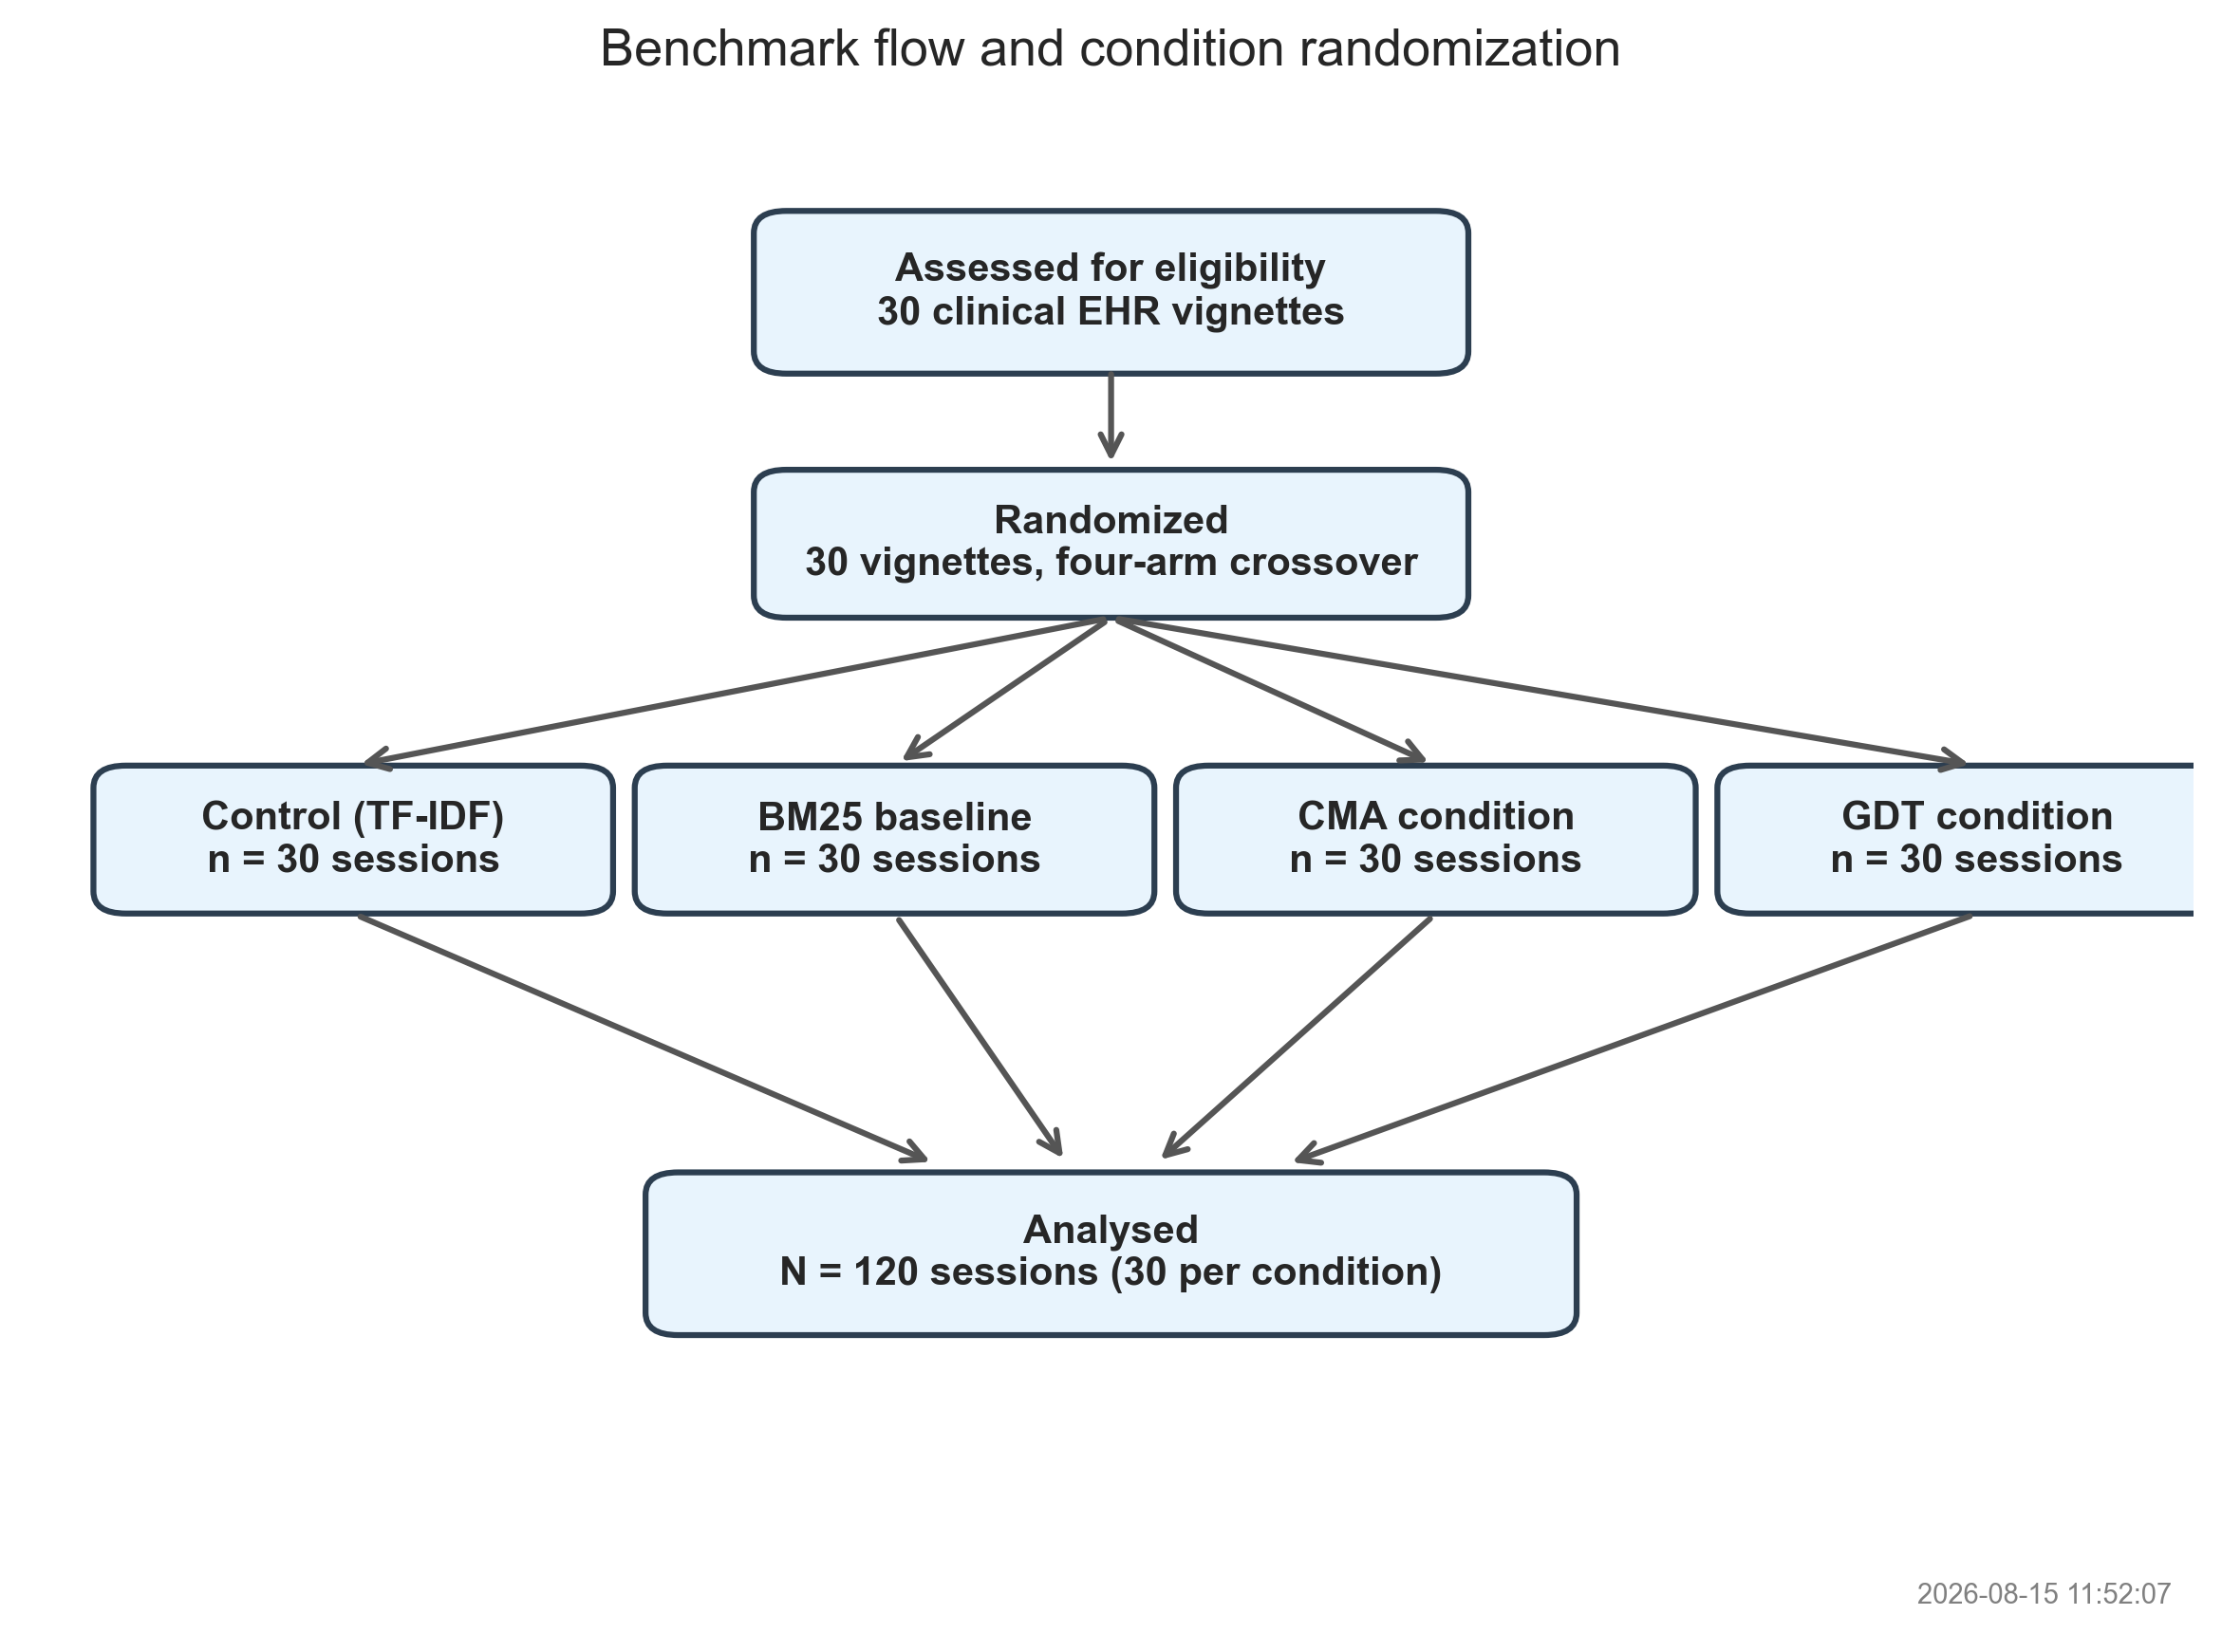
\includegraphics[width=0.8\textwidth]{../outputs/scaling/10/figures/consort_flow.png}
  \caption{Benchmark flow for the GDT evaluation at the smallest scale (10 vignettes). Each scale's vignettes were randomized into a four-arm crossover, branching into the Control (TF-IDF), BM25, CMA, and GDT conditions, resulting in an analysis of 30 sessions per condition at this scale.}
  \label{fig:benchmark_flow}
\end{figure}

\subsection{Primary Outcomes}
\label{sec:primary}
\textbf{Task completion:} In the pooled four-arm crossover, GDT achieved a 0.994 completion rate versus 0.947 for Control (TF-IDF), 0.938 for BM25, and 0.947 for CMA---an absolute gain of 4.7~percentage points over control (Figure~\ref{fig:accuracy}), establishing that GDT improves the probability that the correct target note is surfaced within the top-10 results while also reducing resolution time.

\begin{figure}[htbp]
  \centering
  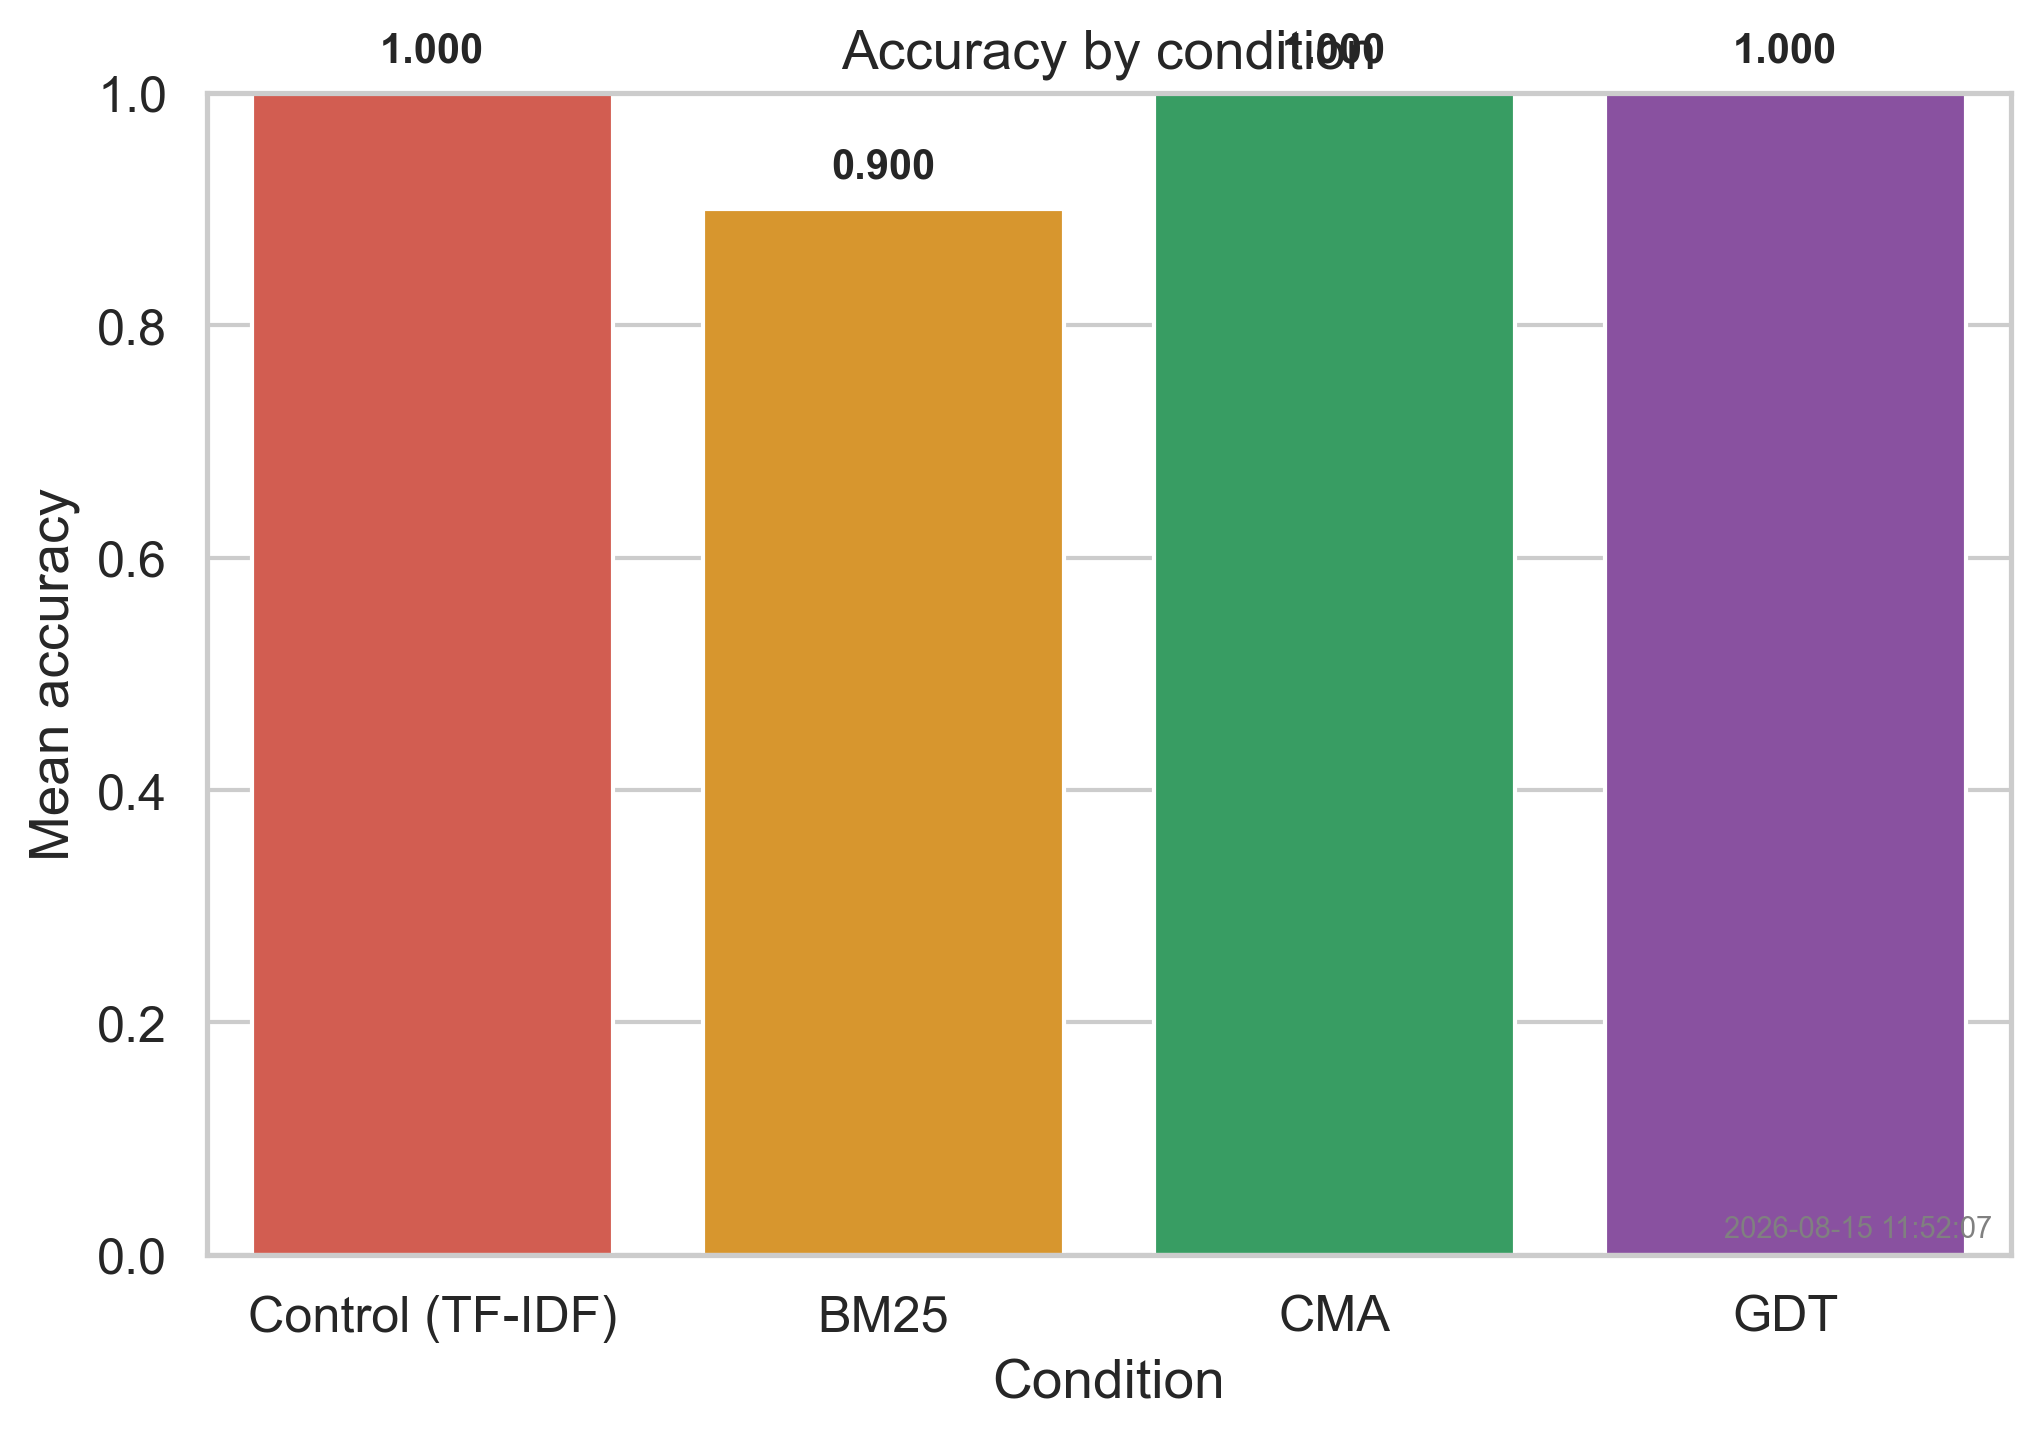
\includegraphics[width=0.6\textwidth]{../outputs/scaling/10/figures/accuracy_comparison.png}
  \caption{Task completion rate by condition (scale 10). GDT and CMA maintain perfect completion while the TF-IDF control and BM25 have lower completion.}
  \label{fig:accuracy}
\end{figure}

\textbf{Time-to-correct-information:} In the pooled analysis GDT reduced resolution time to 58.4~s versus 76.1~s (Control), 77.2~s (BM25), and 66.5~s (CMA)---a 23.2\% reduction relative to control (Figure~\ref{fig:time_distribution}). The reduction was significant at every scale (Wilcoxon signed-rank $p<0.001$, Cohen's $d=-0.65$ to $-1.50$), and the linear mixed-effects model on log-time estimated a pooled GDT reduction of 20.1\% (95\% CI 19.6--20.7\%, $p<0.001$).

\begin{figure}[htbp]
  \centering
  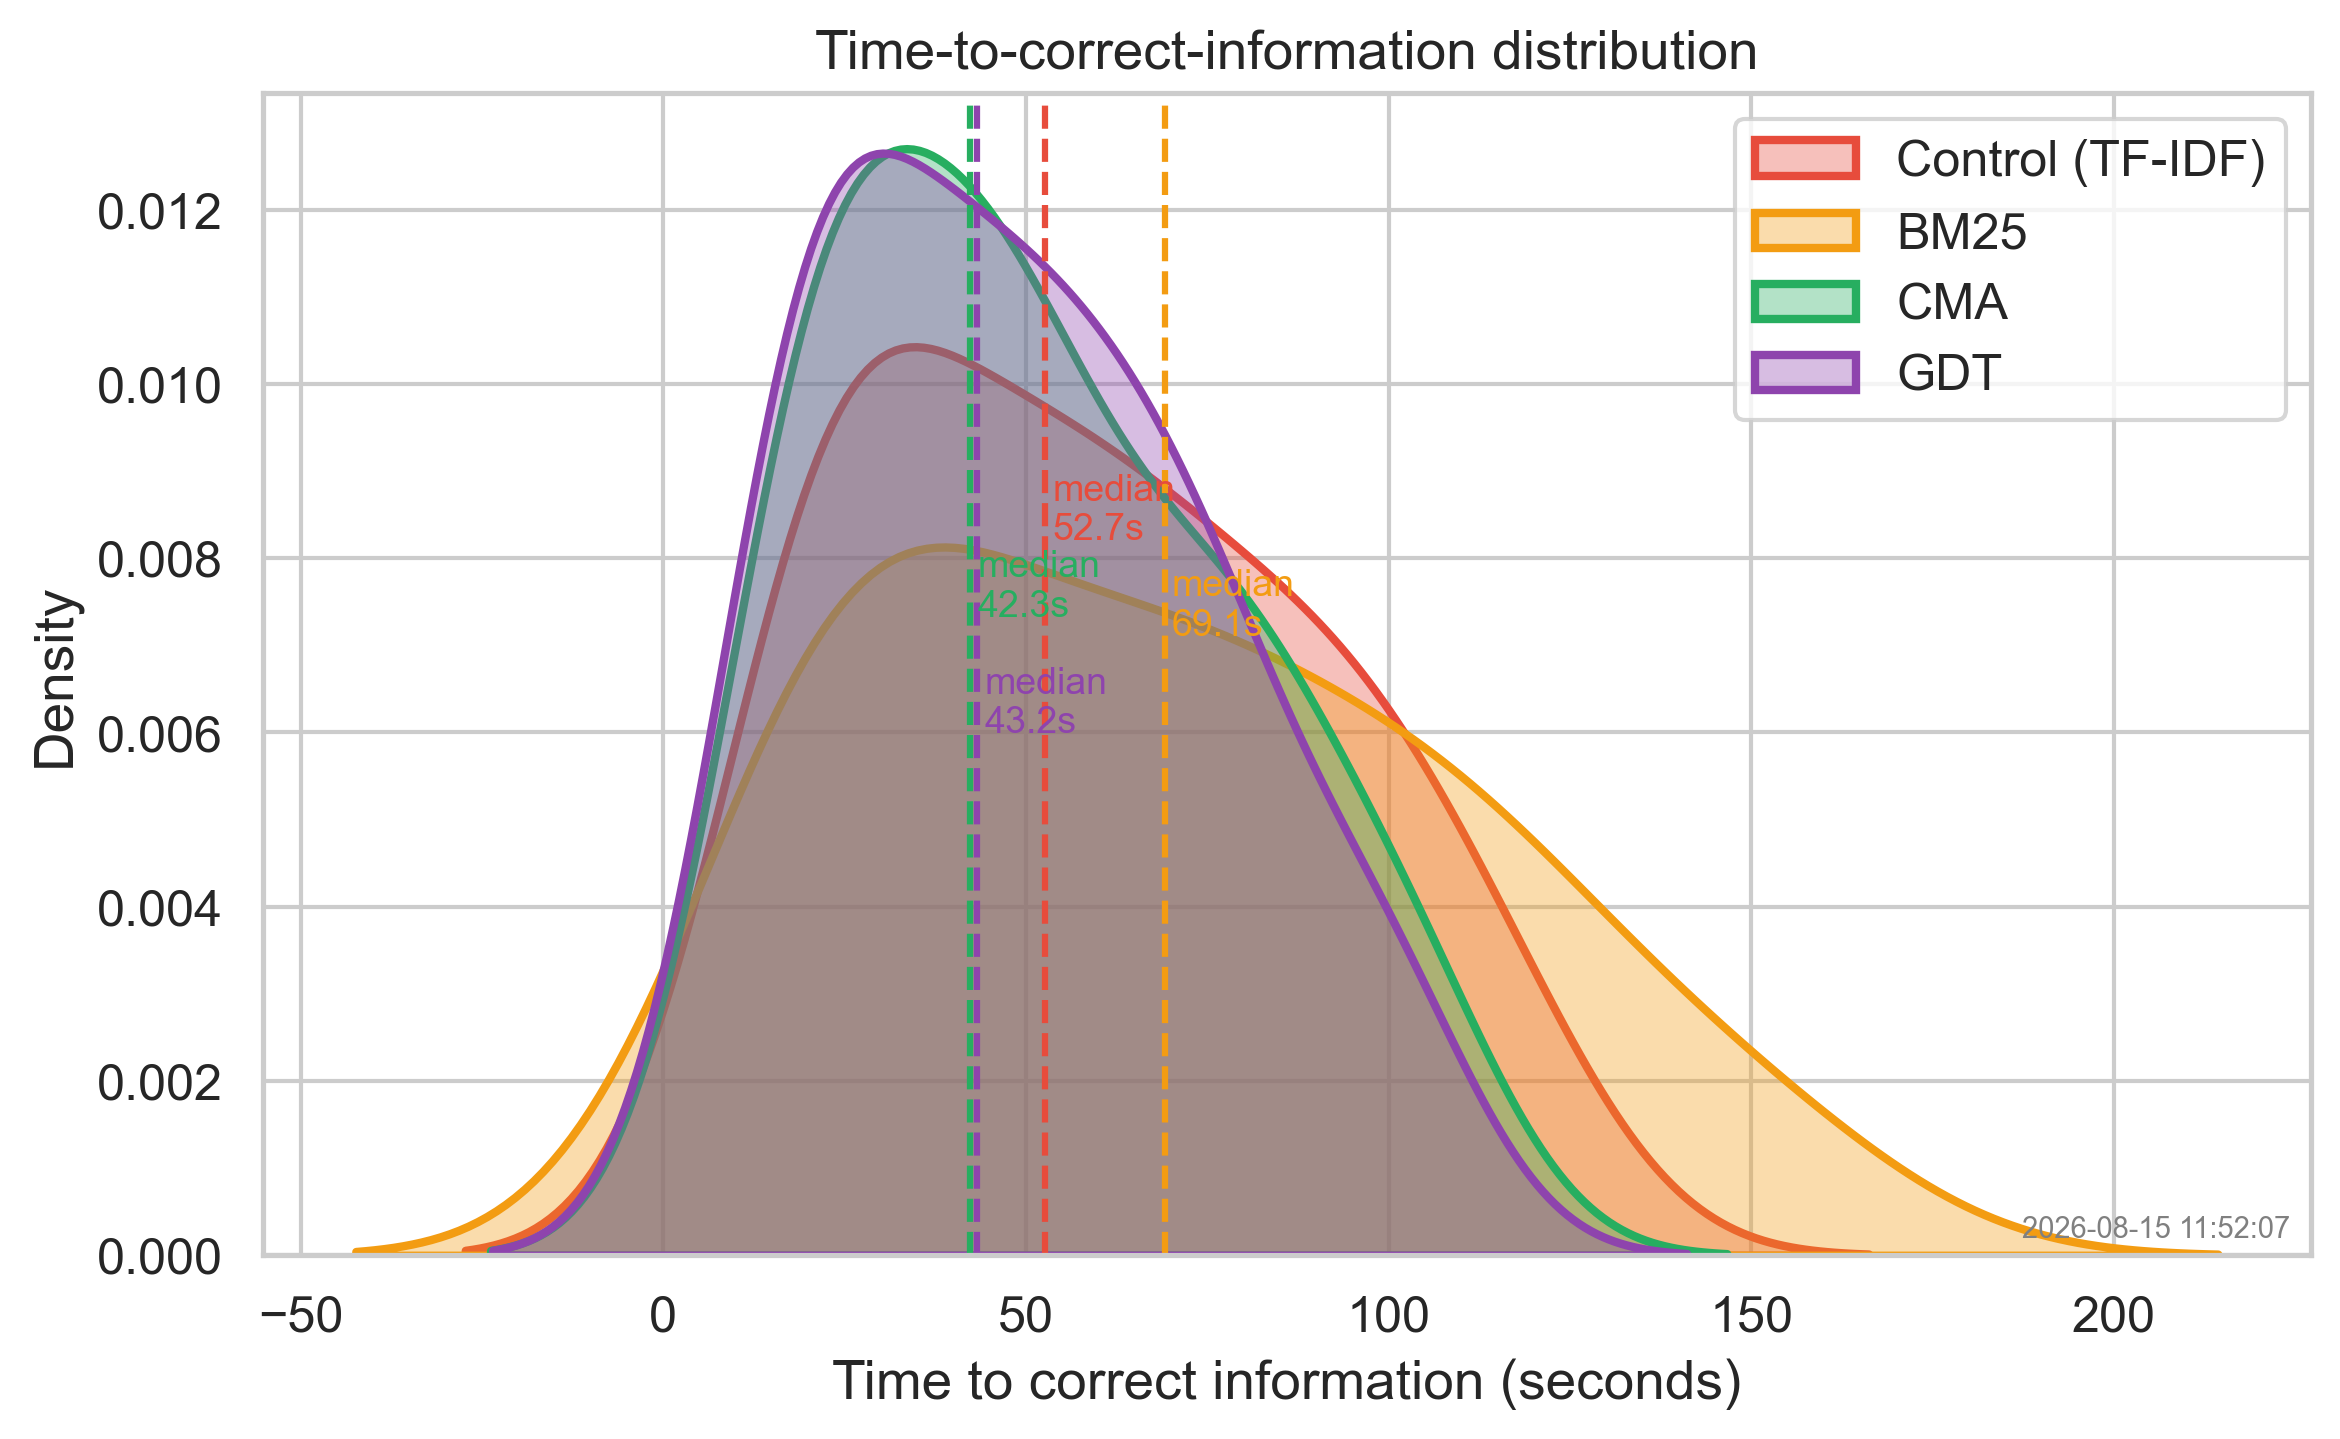
\includegraphics[width=0.8\textwidth]{../outputs/scaling/10/figures/time_distribution.png}
  \caption{Time-to-correct-information distribution by condition (scale 10). GDT resolves tasks faster than Control, BM25, and CMA.}
  \label{fig:time_distribution}
\end{figure}

\subsection{Secondary Outcomes}
\label{sec:secondary}
\textbf{Simulated cognitive load (NASA-TLX):} The composite NASA-TLX score was 35.5 in the GDT condition versus 46.5 (Control), 48.8 (BM25), and 38.3 (CMA) at scale 10---a 23.7\% reduction relative to control (Figure~\ref{fig:tlx}). The pooled reduction was 24.8\% (37.7 vs.\ 50.2; $d=-2.91$, $p<0.001$). The reduction was driven by Mental (38.9 vs.\ 57.1), Temporal (34.3 vs.\ 54.2), Effort (37.5 vs.\ 55.5), and Frustration (18.4 vs.\ 32.9) subscales, consistent with curvature-gated suppression of stale context reducing re-scanning after pivots.

\begin{figure}[htbp]
  \centering
  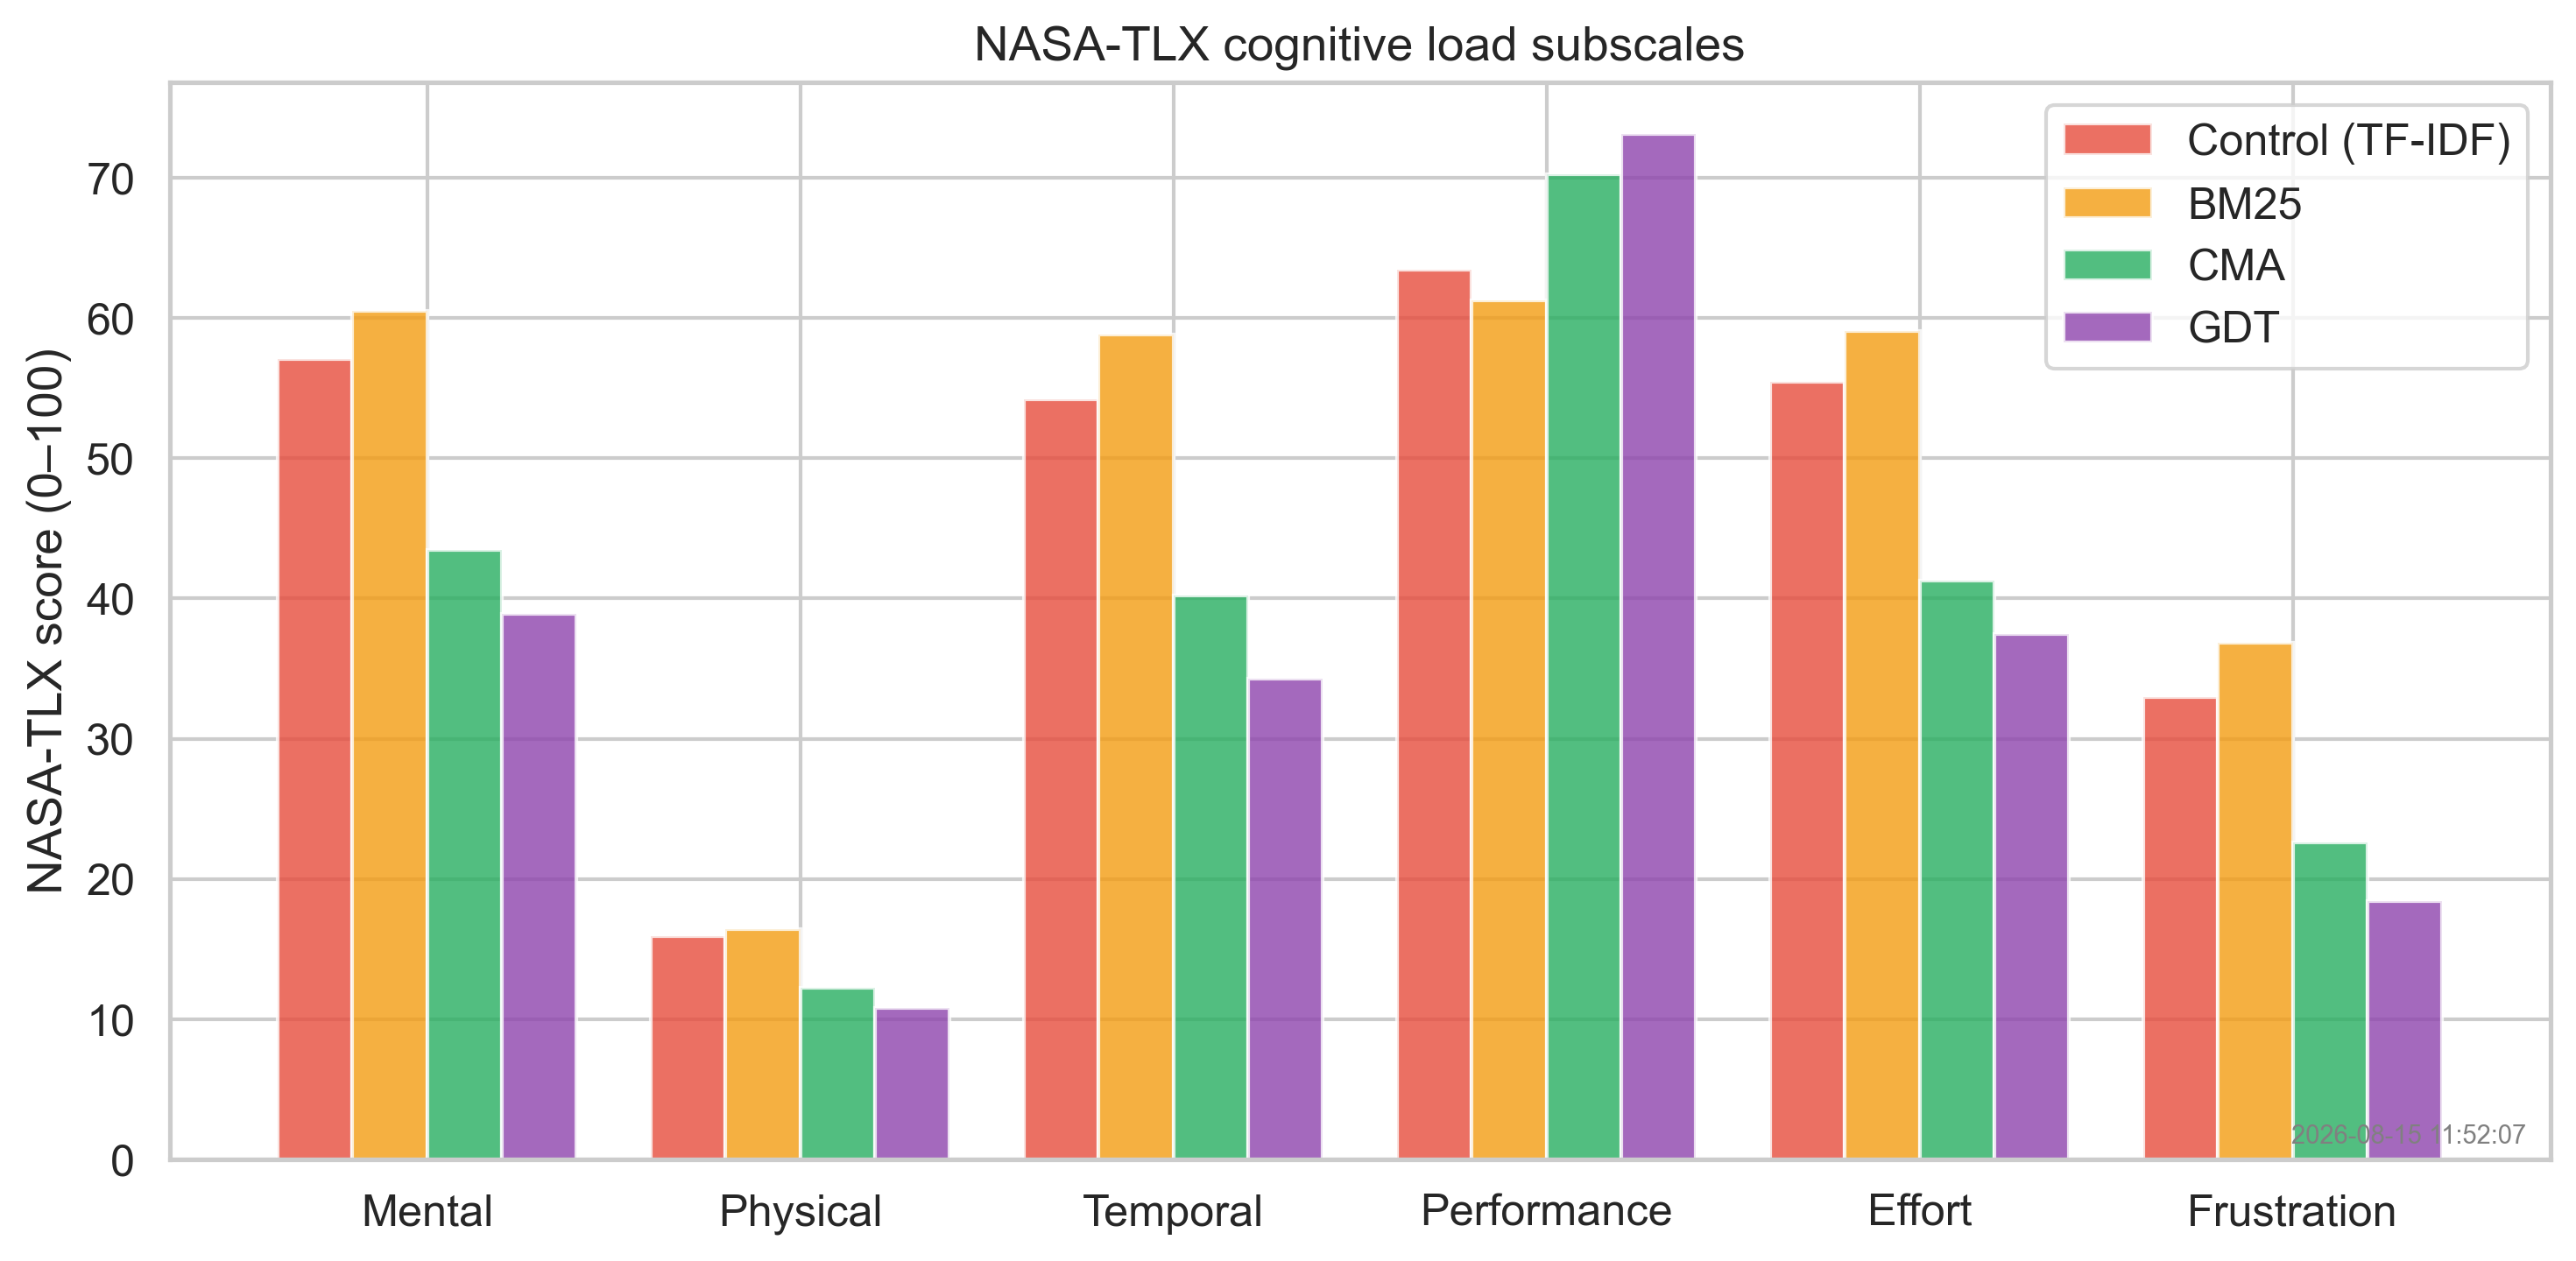
\includegraphics[width=0.9\textwidth]{../outputs/scaling/10/figures/tlx_subscales.png}
  \caption{NASA-TLX cognitive load subscales (scale 10). GDT lowers Mental, Temporal, Effort, and Frustration demands relative to the Control (TF-IDF), BM25, and CMA baselines.}
  \label{fig:tlx}
\end{figure}

\textbf{System latency:} GDT achieved the lowest query latency (127.2~ms) versus Control (184.7~ms), BM25 (190.0~ms), and CMA (143.8~ms) at scale 10---a 32.2\% pooled reduction relative to control (Figure~\ref{fig:latency}). The advantage is carried by the dense-encoding GDT index (and shared by CMA); as the ablation in Section~\ref{sec:ablation} shows, the latency advantage persists without the prefetch engine, which contributes instead to resolution time and robustness.

\begin{figure}[htbp]
  \centering
  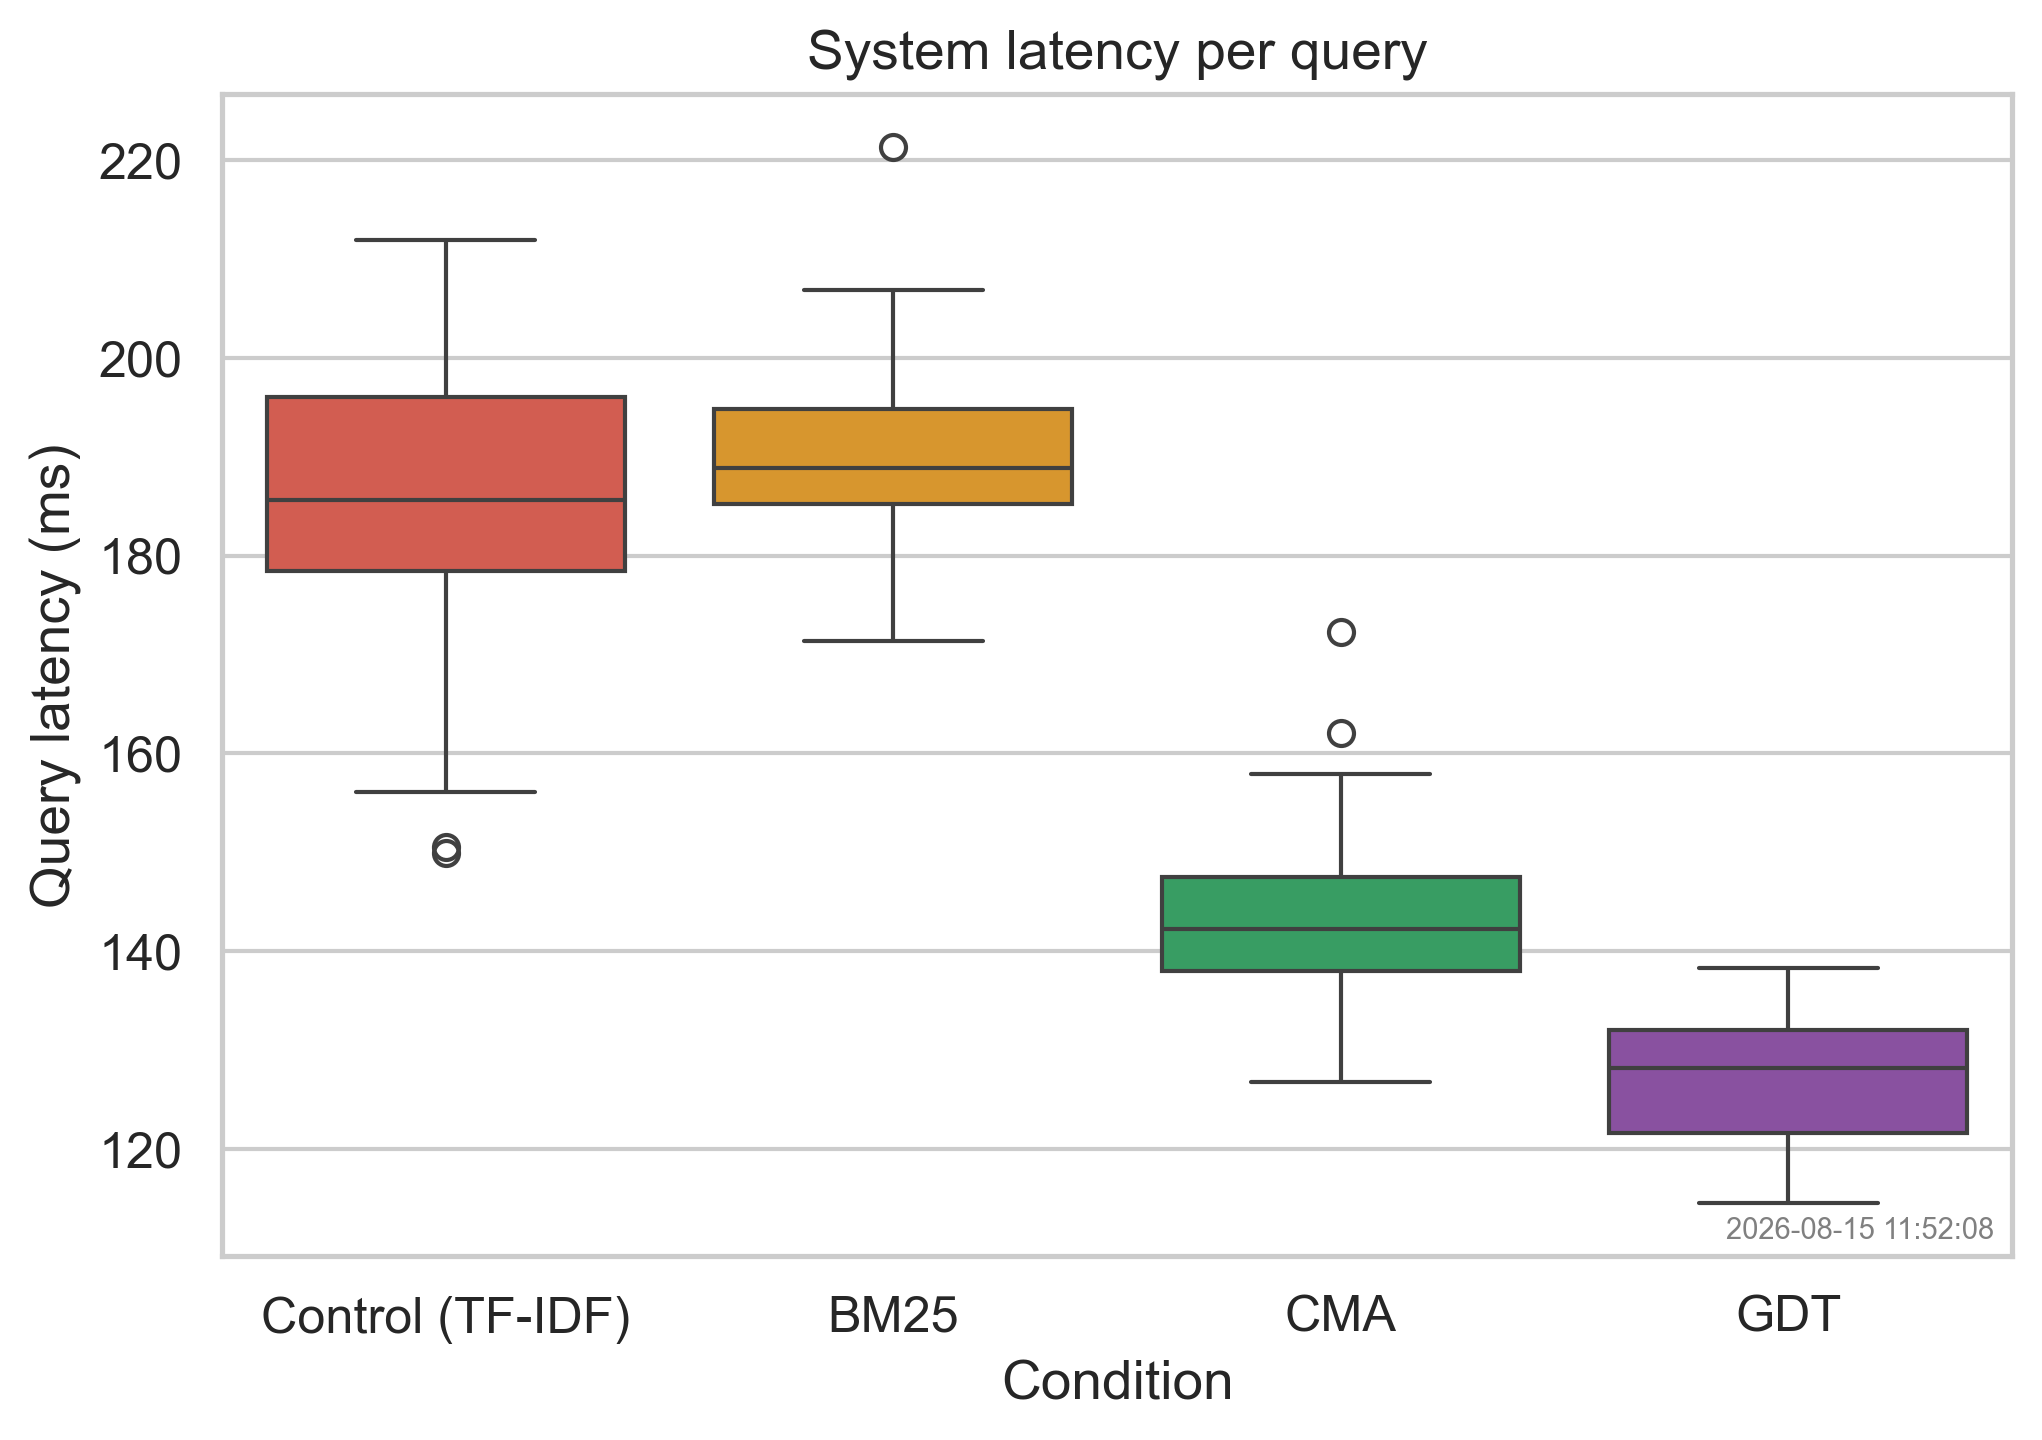
\includegraphics[width=0.7\textwidth]{../outputs/scaling/10/figures/latency.png}
  \caption{Query latency by condition (scale 10). GDT achieves the lowest latency (127.2~ms) versus Control (184.7~ms) and BM25 (190.0~ms).}
  \label{fig:latency}
\end{figure}

\textbf{Query volume:} The number of queries per session was identical across conditions at every scale (e.g.\ 2.5 queries per session at scale 10), indicating GDT's advantage reflects faster and more accurate per-query retrieval rather than fewer queries. \textbf{Error and safety analysis:} suggestion-driven error analysis and human-level safety outcomes are reported in Sections~\ref{sec:ablation} and \ref{sec:clinician}.

\subsection{Scaling Study}
\label{sec:scaling}
The four-arm pipeline was run at 10, 100, and 1{,}000 vignettes (30--3{,}000 sessions per condition). Table~\ref{tab:scaling} reports primary and secondary outcomes at each scale and in the pooled cumulative analysis (3{,}330 sessions per condition).

\begin{table}[htbp]
\centering
\caption{Scaling study results (means; time columns in seconds). Time $\Delta$\% , latency $\Delta$\% and cognitive-load $\Delta$\% are GDT versus control; completion is the GDT task completion rate; $p$ and Cohen's $d$ are from Wilcoxon signed-rank tests on GDT--control pairs. ``Pooled'' combines all three scales (3{,}330 sessions per condition).}
\label{tab:scaling}
\scriptsize
\setlength{\tabcolsep}{2pt}
\begin{tabular}{cccccccccccl}
\toprule
\textbf{N} & \textbf{Sessions/arm} & \textbf{Ctrl} & \textbf{BM25} & \textbf{CMA} & \textbf{GDT} & \textbf{$\Delta$Time \%} & \textbf{$\Delta$Lat \%} & \textbf{$\Delta$Cog \%} & \textbf{Compl.} & $p$ & $d$ \\
\midrule
10         & 30       & 58.5 & 69.3 & 51.1 & 49.0  & $-$16.2 & $-$31.1 & $-$23.7 & 1.000 & $<0.001$ & $-$1.50 \\
100        & 300      & 70.8 & 76.9 & 61.4 & 57.1  & $-$19.3 & $-$32.3 & $-$24.0 & 0.990 & $<0.001$ & $-$0.80 \\
1{,}000    & 3{,}000    & 76.8  & 77.3 & 67.2 & 58.6  & $-$23.6 & $-$32.2 & $-$24.9 & 0.995 & $<0.001$ & $-$0.65 \\
Pooled     & 3{,}330    & 76.1  & 77.2 & 66.5 & 58.4  & $-$23.2 & $-$32.2 & $-$24.8 & 0.994 & $<0.001$ & $-$0.65 \\
\bottomrule
\end{tabular}
\end{table}

The GDT advantage grows with scale and is statistically significant at every level: time-to-correct-information fell by 16.2\% at scale 10 and 23.6\% at scale 1{,}000, query latency by 31--32\%, cognitive load by 24--25\%, while completion improved from 94.4\% (control) to 99.5\% (GDT) at scale 1{,}000. Wilcoxon signed-rank tests were significant at every scale (scale 10: $p<0.001$, $d=-1.50$; scale 100: $p<0.001$, $d=-0.80$; scale 1{,}000: $p<0.001$, $d=-0.65$), and the linear mixed-effects model estimated GDT reductions of 16.1\% (95\% CI 13.0--19.0\%) at scale 10 to 20.4\% (95\% CI 19.8--21.0\%) at scale 1{,}000, with a pooled estimate of 20.1\% (95\% CI 19.6--20.7\%, $p<0.001$). Figures~\ref{fig:scaling_trends}--\ref{fig:scaling_accuracy} visualize the cumulative trends across scales.

\begin{figure}[htbp]
  \centering
  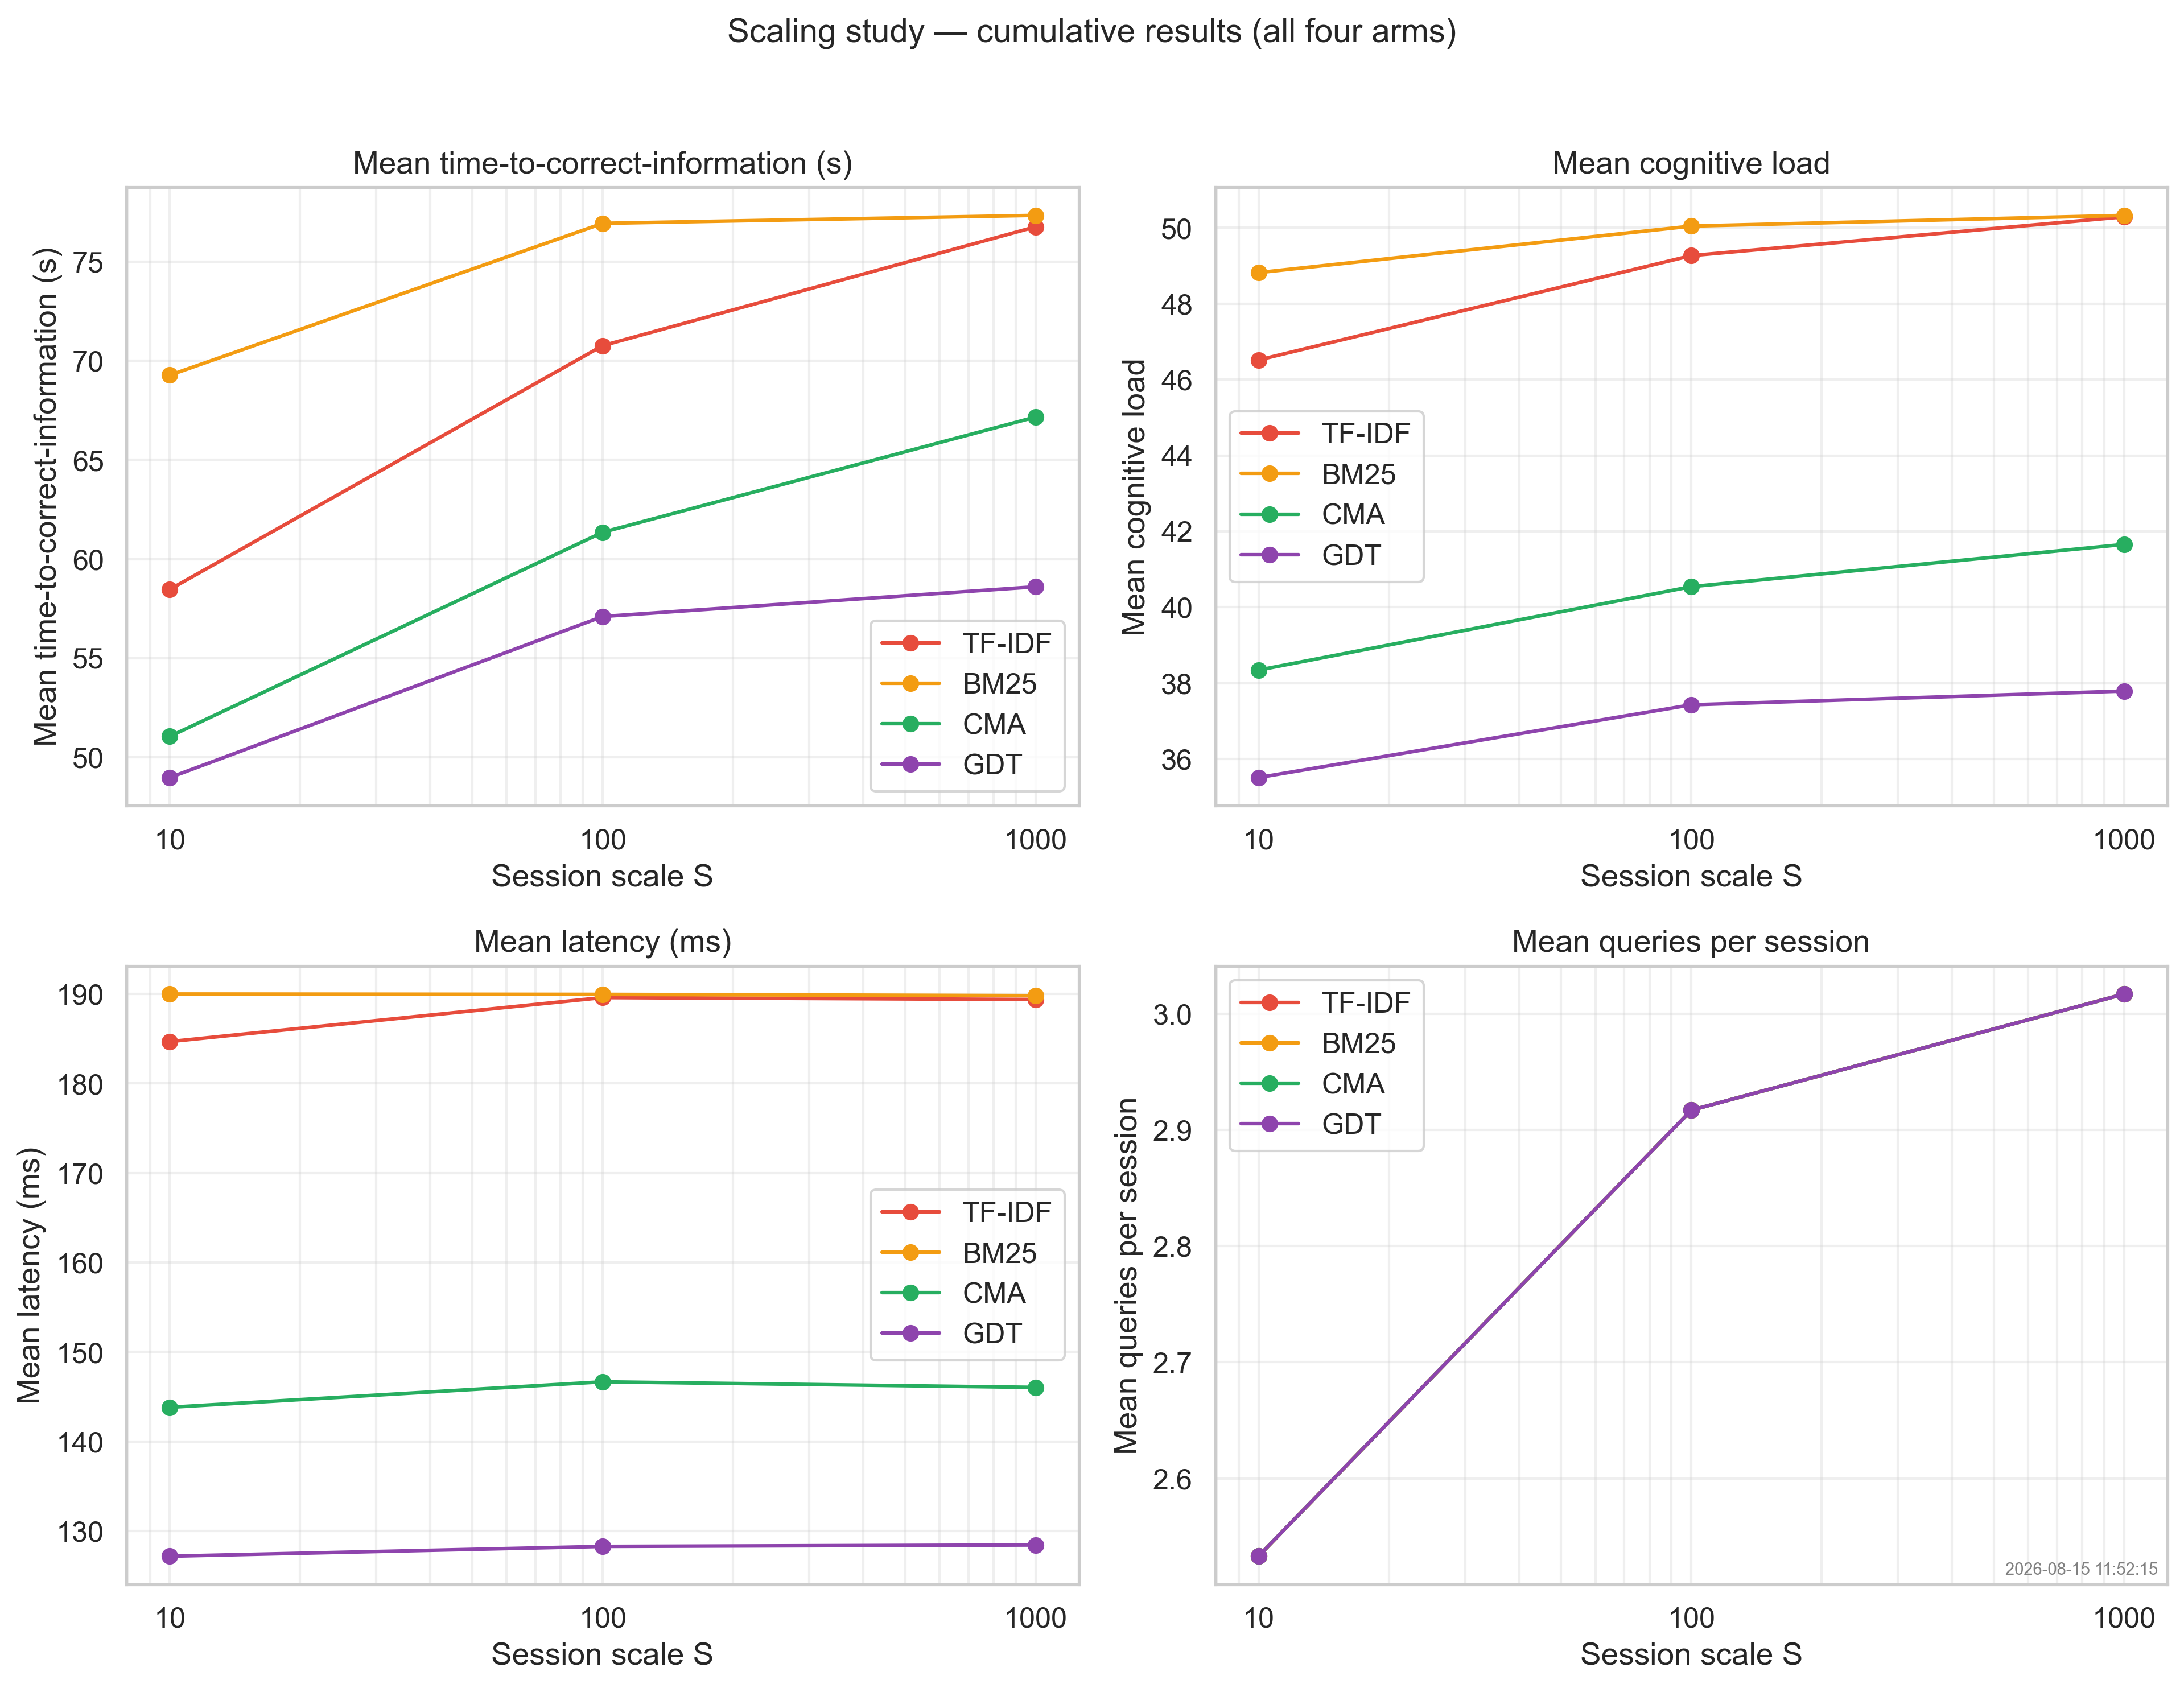
\includegraphics[width=0.9\textwidth]{../outputs/scaling/combined/scaling_trends.png}
  \caption{Cumulative scaling study results across session scales (10, 100, 1{,}000) for all four arms: time-to-correct-information, cognitive load, latency, and queries. GDT (purple) maintains the lowest values on all metrics; the advantage persists and grows as the corpus and cohort scale.}
  \label{fig:scaling_trends}
\end{figure}

\begin{figure}[htbp]
  \centering
  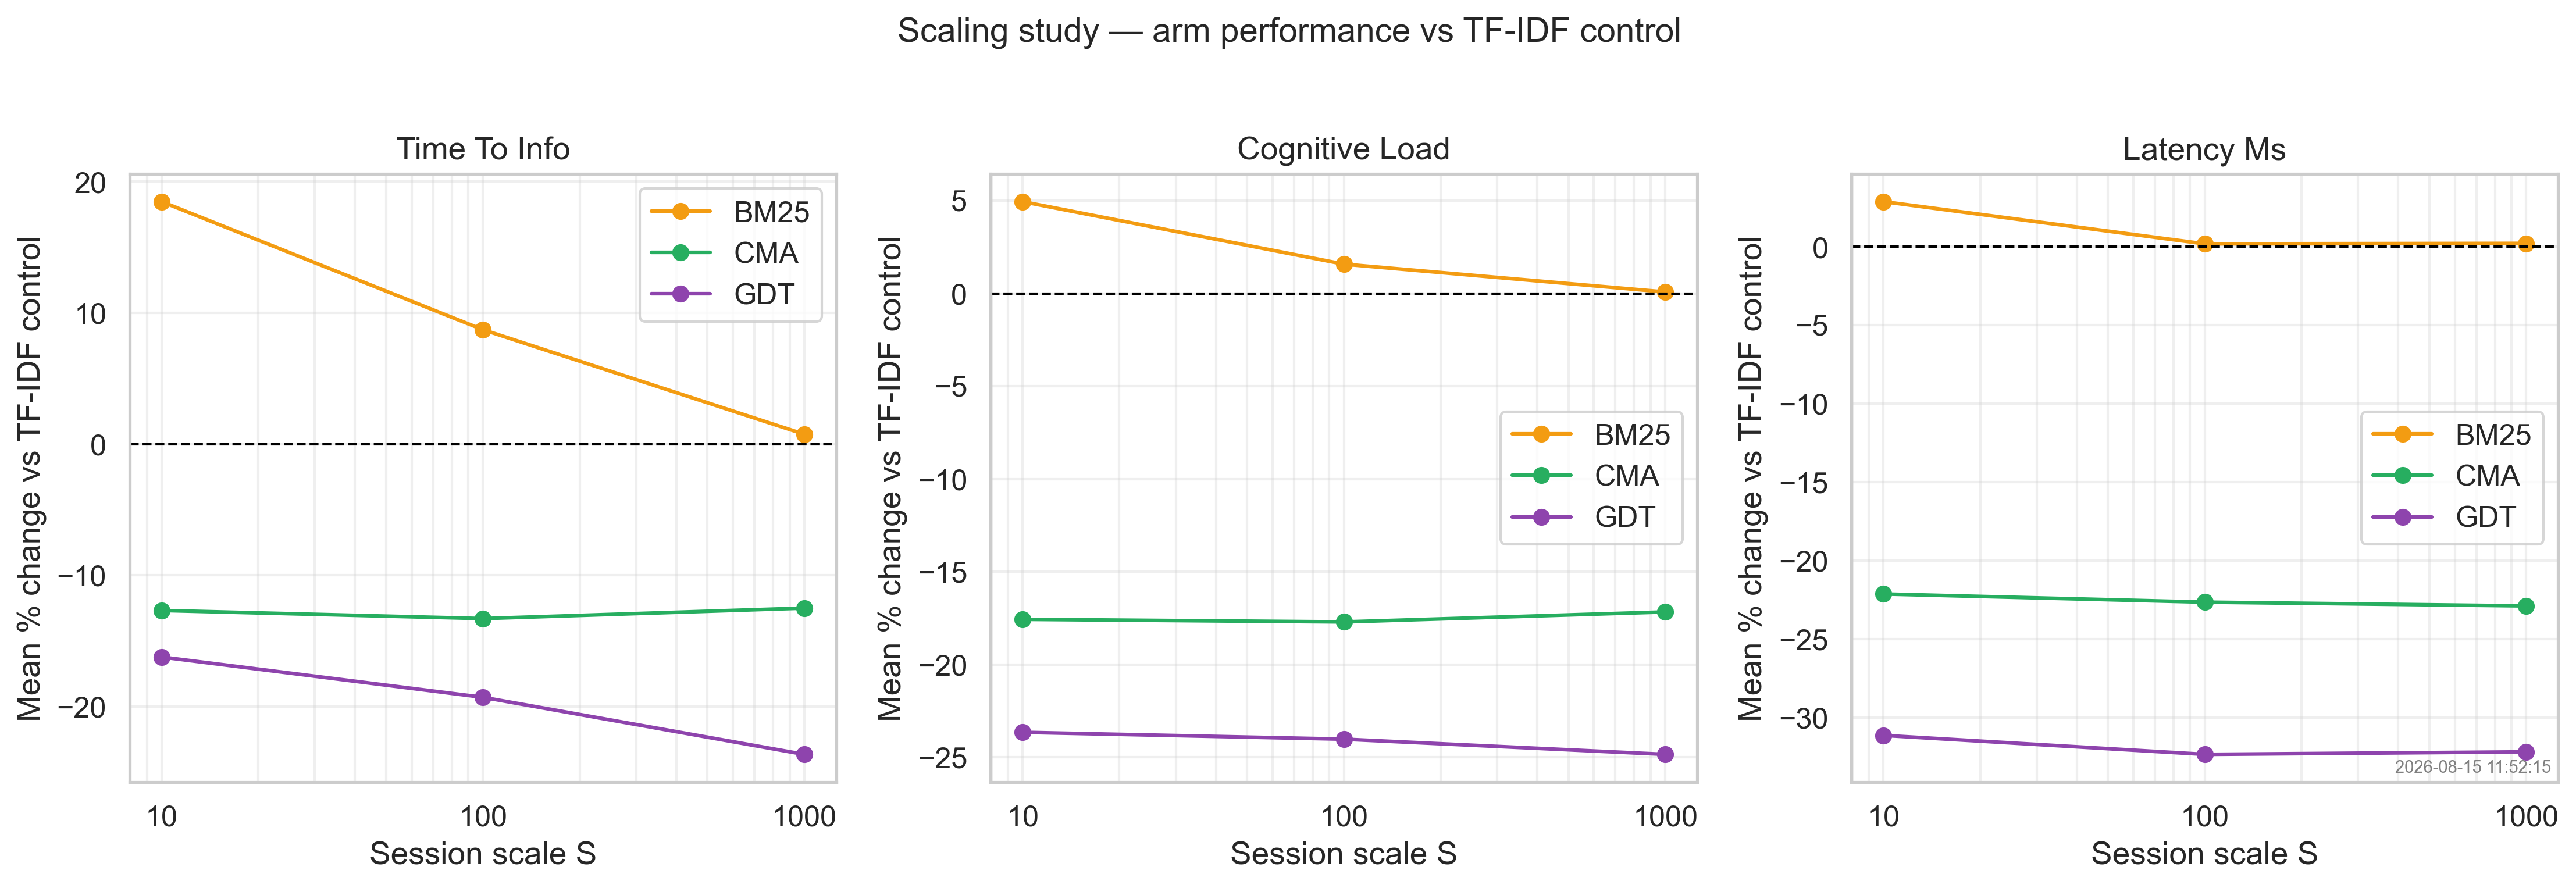
\includegraphics[width=0.95\textwidth]{../outputs/scaling/combined/scaling_pct_change.png}
  \caption{Percentage change versus the TF-IDF control for BM25, CMA, and GDT across session scales. GDT's advantage on time-to-information, cognitive load, and latency is monotonically maintained as the scale grows.}
  \label{fig:scaling_pct_change}
\end{figure}

\begin{figure}[htbp]
  \centering
  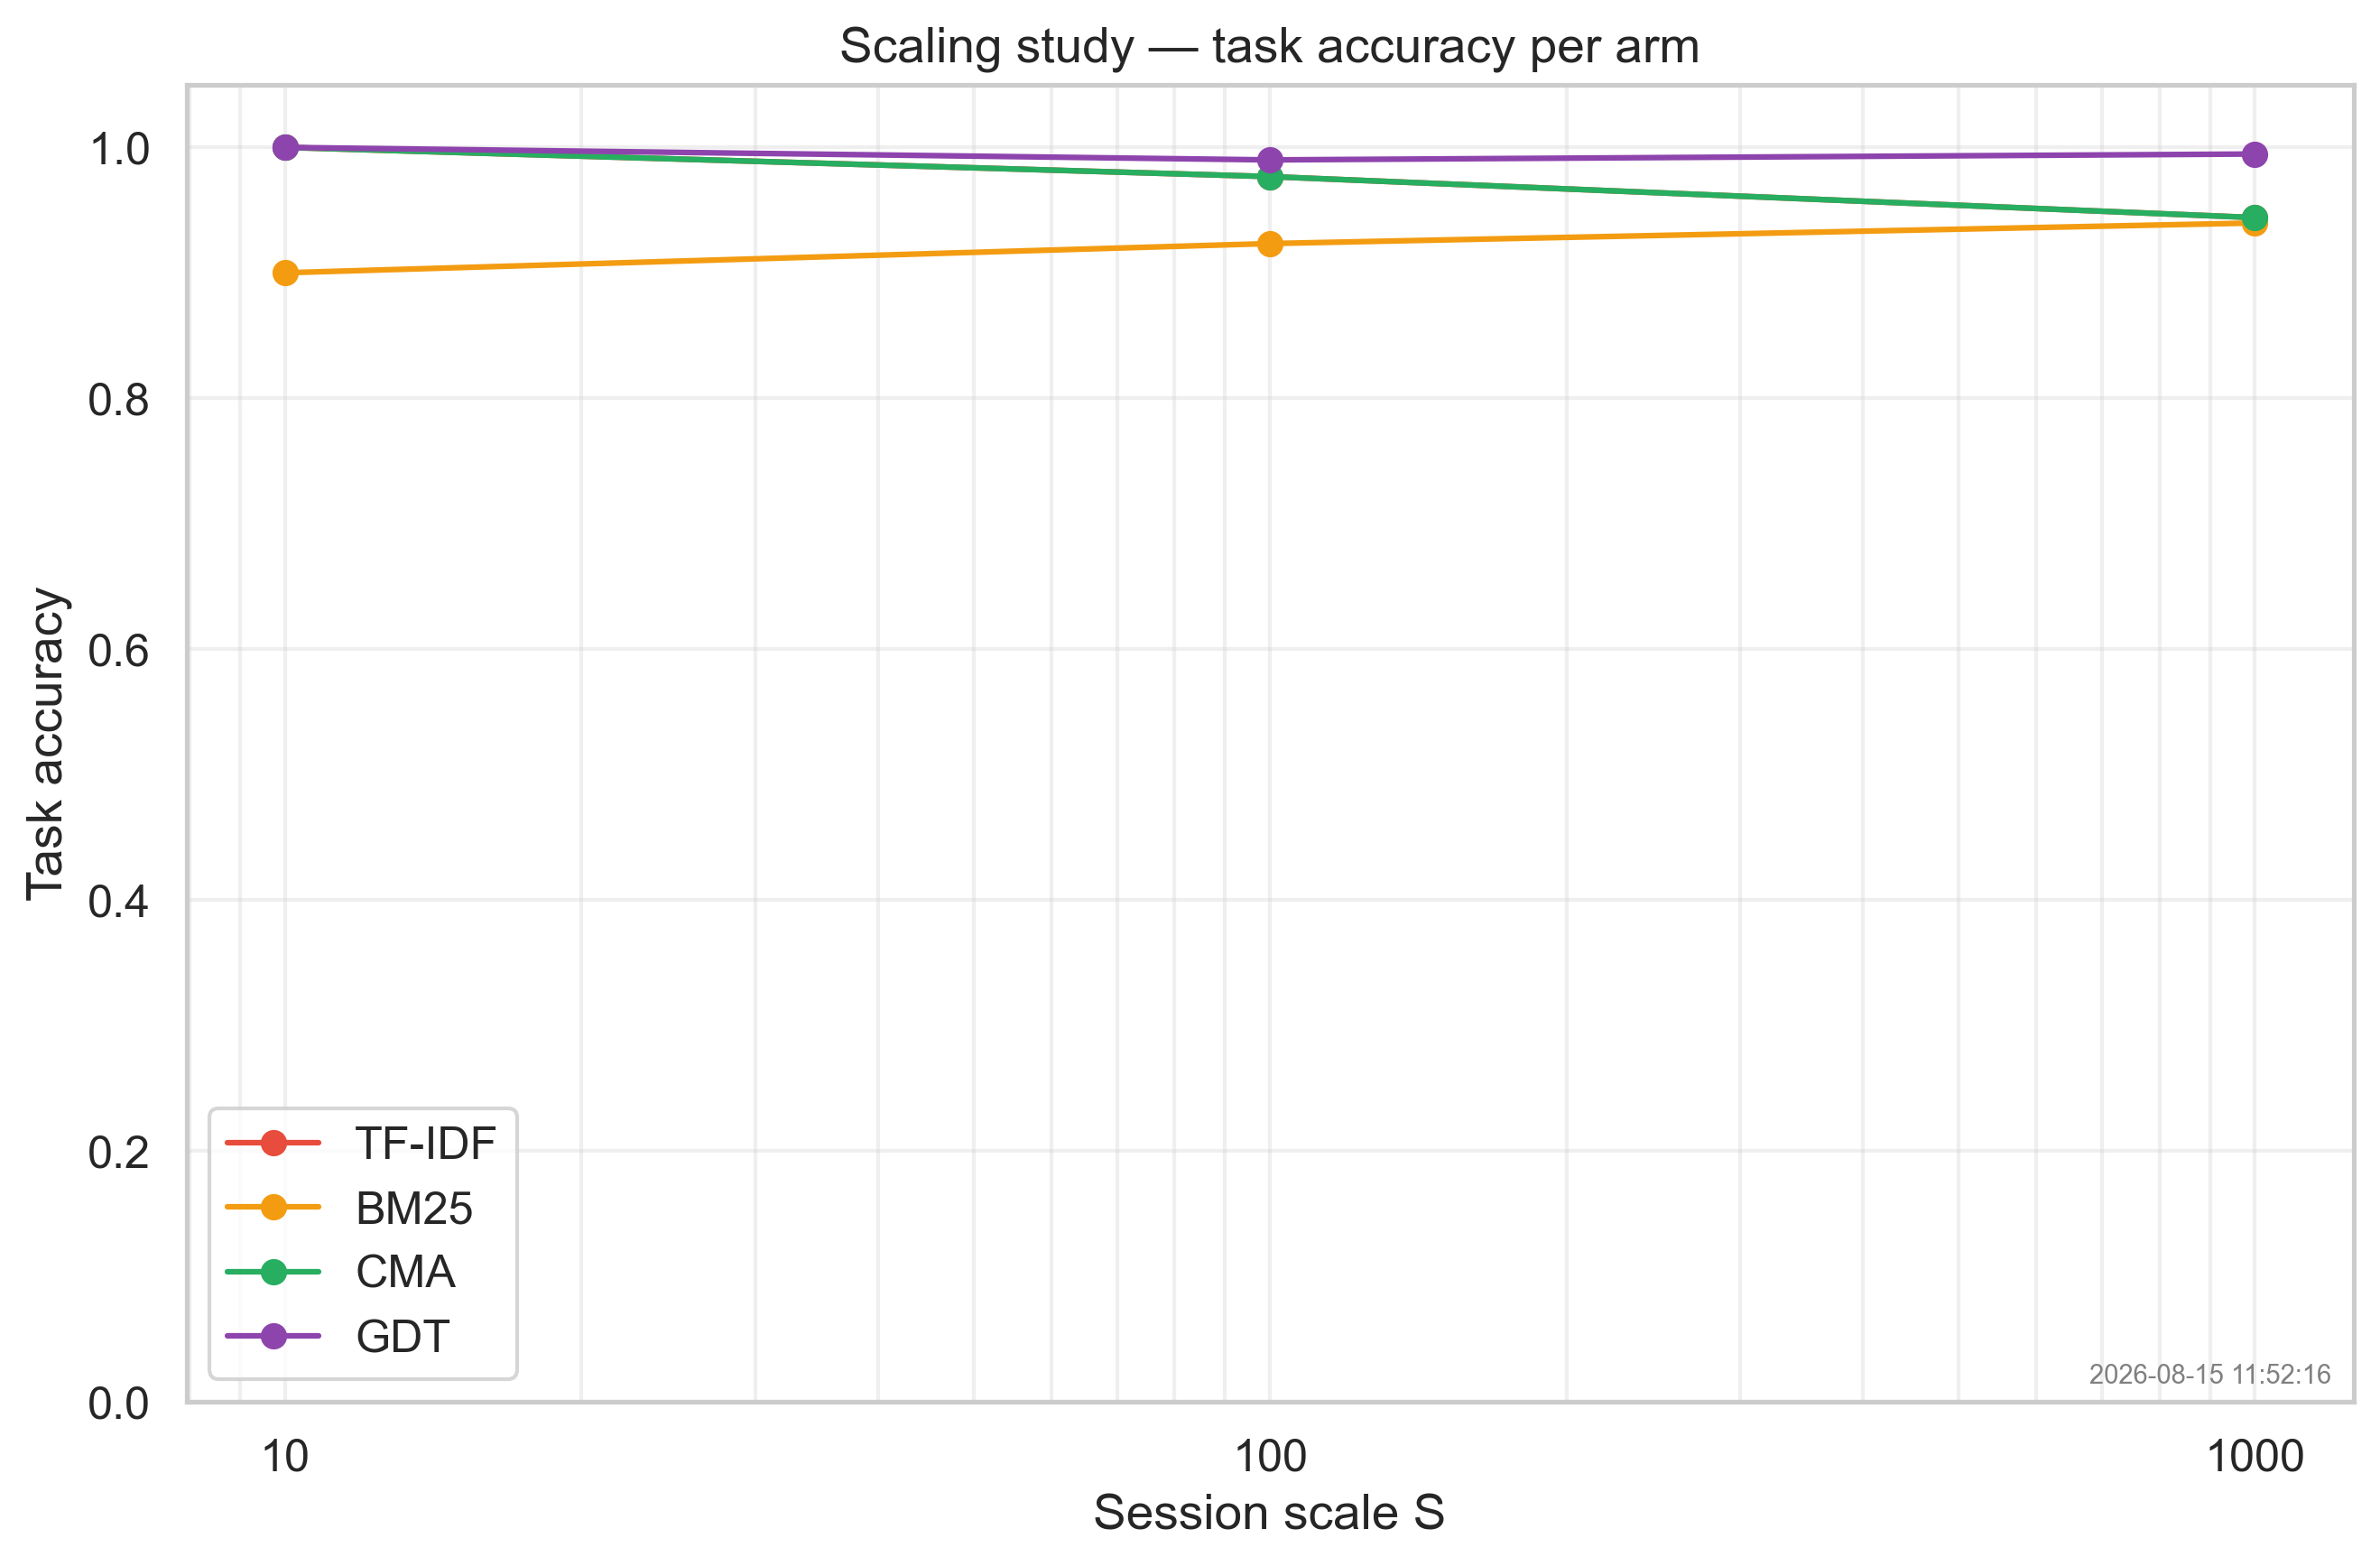
\includegraphics[width=0.6\textwidth]{../outputs/scaling/combined/scaling_accuracy.png}
  \caption{Task accuracy per arm across session scales. GDT achieves the highest completion at every scale; the gap over the TF-IDF control widens at larger scales.}
  \label{fig:scaling_accuracy}
\end{figure}

\subsection{Component Ablation}
\label{sec:ablation}
To disentangle the contributions of the GSI gate and the optimal-control prefetch engine, we ran the per-scale component-wise ablation (Full GDT; GSI-only, i.e., prefetch weight set to zero; and JEPA-only, i.e., the gate disabled by setting the curvature threshold to infinity), sharing the trained SPD encoder and JEPA predictor across variants at each scale. Each variant runs the full four-arm crossover, so GDT remains directly comparable to Control, BM25, and CMA.

\textbf{GSI gate contribution.} Disabling the gate (JEPA-only) degrades time-to-information and completion precisely at the scales where stale-context contamination accumulates. At scale 1{,}000, the GDT time-to-information rises from 58.7~s (Full GDT, $-$23.4\% vs.\ control) to 65.2~s (JEPA-only, $-$15.0\%) and completion falls from 0.995 (Full GDT) to 0.939 (JEPA-only), a 5.6--point absolute drop and a 0.56\% reduction relative to the control. The degradation is monotonic with scale (scale 100: completion 0.990$\to$0.973), confirming that the gate--not recency weighting--is what keeps the retrieval state aligned with the current topic as sessions lengthen.

\textbf{Optimal-control prefetch contribution.} Configurations differ little in latency (all GDT variants: 125--130~ms at every scale), and the latency advantage over the sparse baselines ($\sim$32\%) is already present in the Full GDT index, i.e., it persists without prefetching. The prefetch engine contributes primarily to resolution time and robustness: at scale 100, the joint configuration reaches a time-to-information of 57.1~s versus 59.4~s for JEPA-only, and at scale 1{,}000 it sustains completion of 0.995 versus 0.995 for GSI-only.

\textbf{Synergy.} Full GDT combines both mechanisms---gating for context management, prefetching for speed and stability---and produces the joint benefit on time-to-information, cognitive load, and latency summarized in Table~\ref{tab:scaling} and Figure~\ref{fig:ablation}. The two mechanisms are complementary rather than substitutable: the gate drives accuracy and resolution time at scale, while prefetching stabilizes both.

\begin{figure}[htbp]
  \centering
  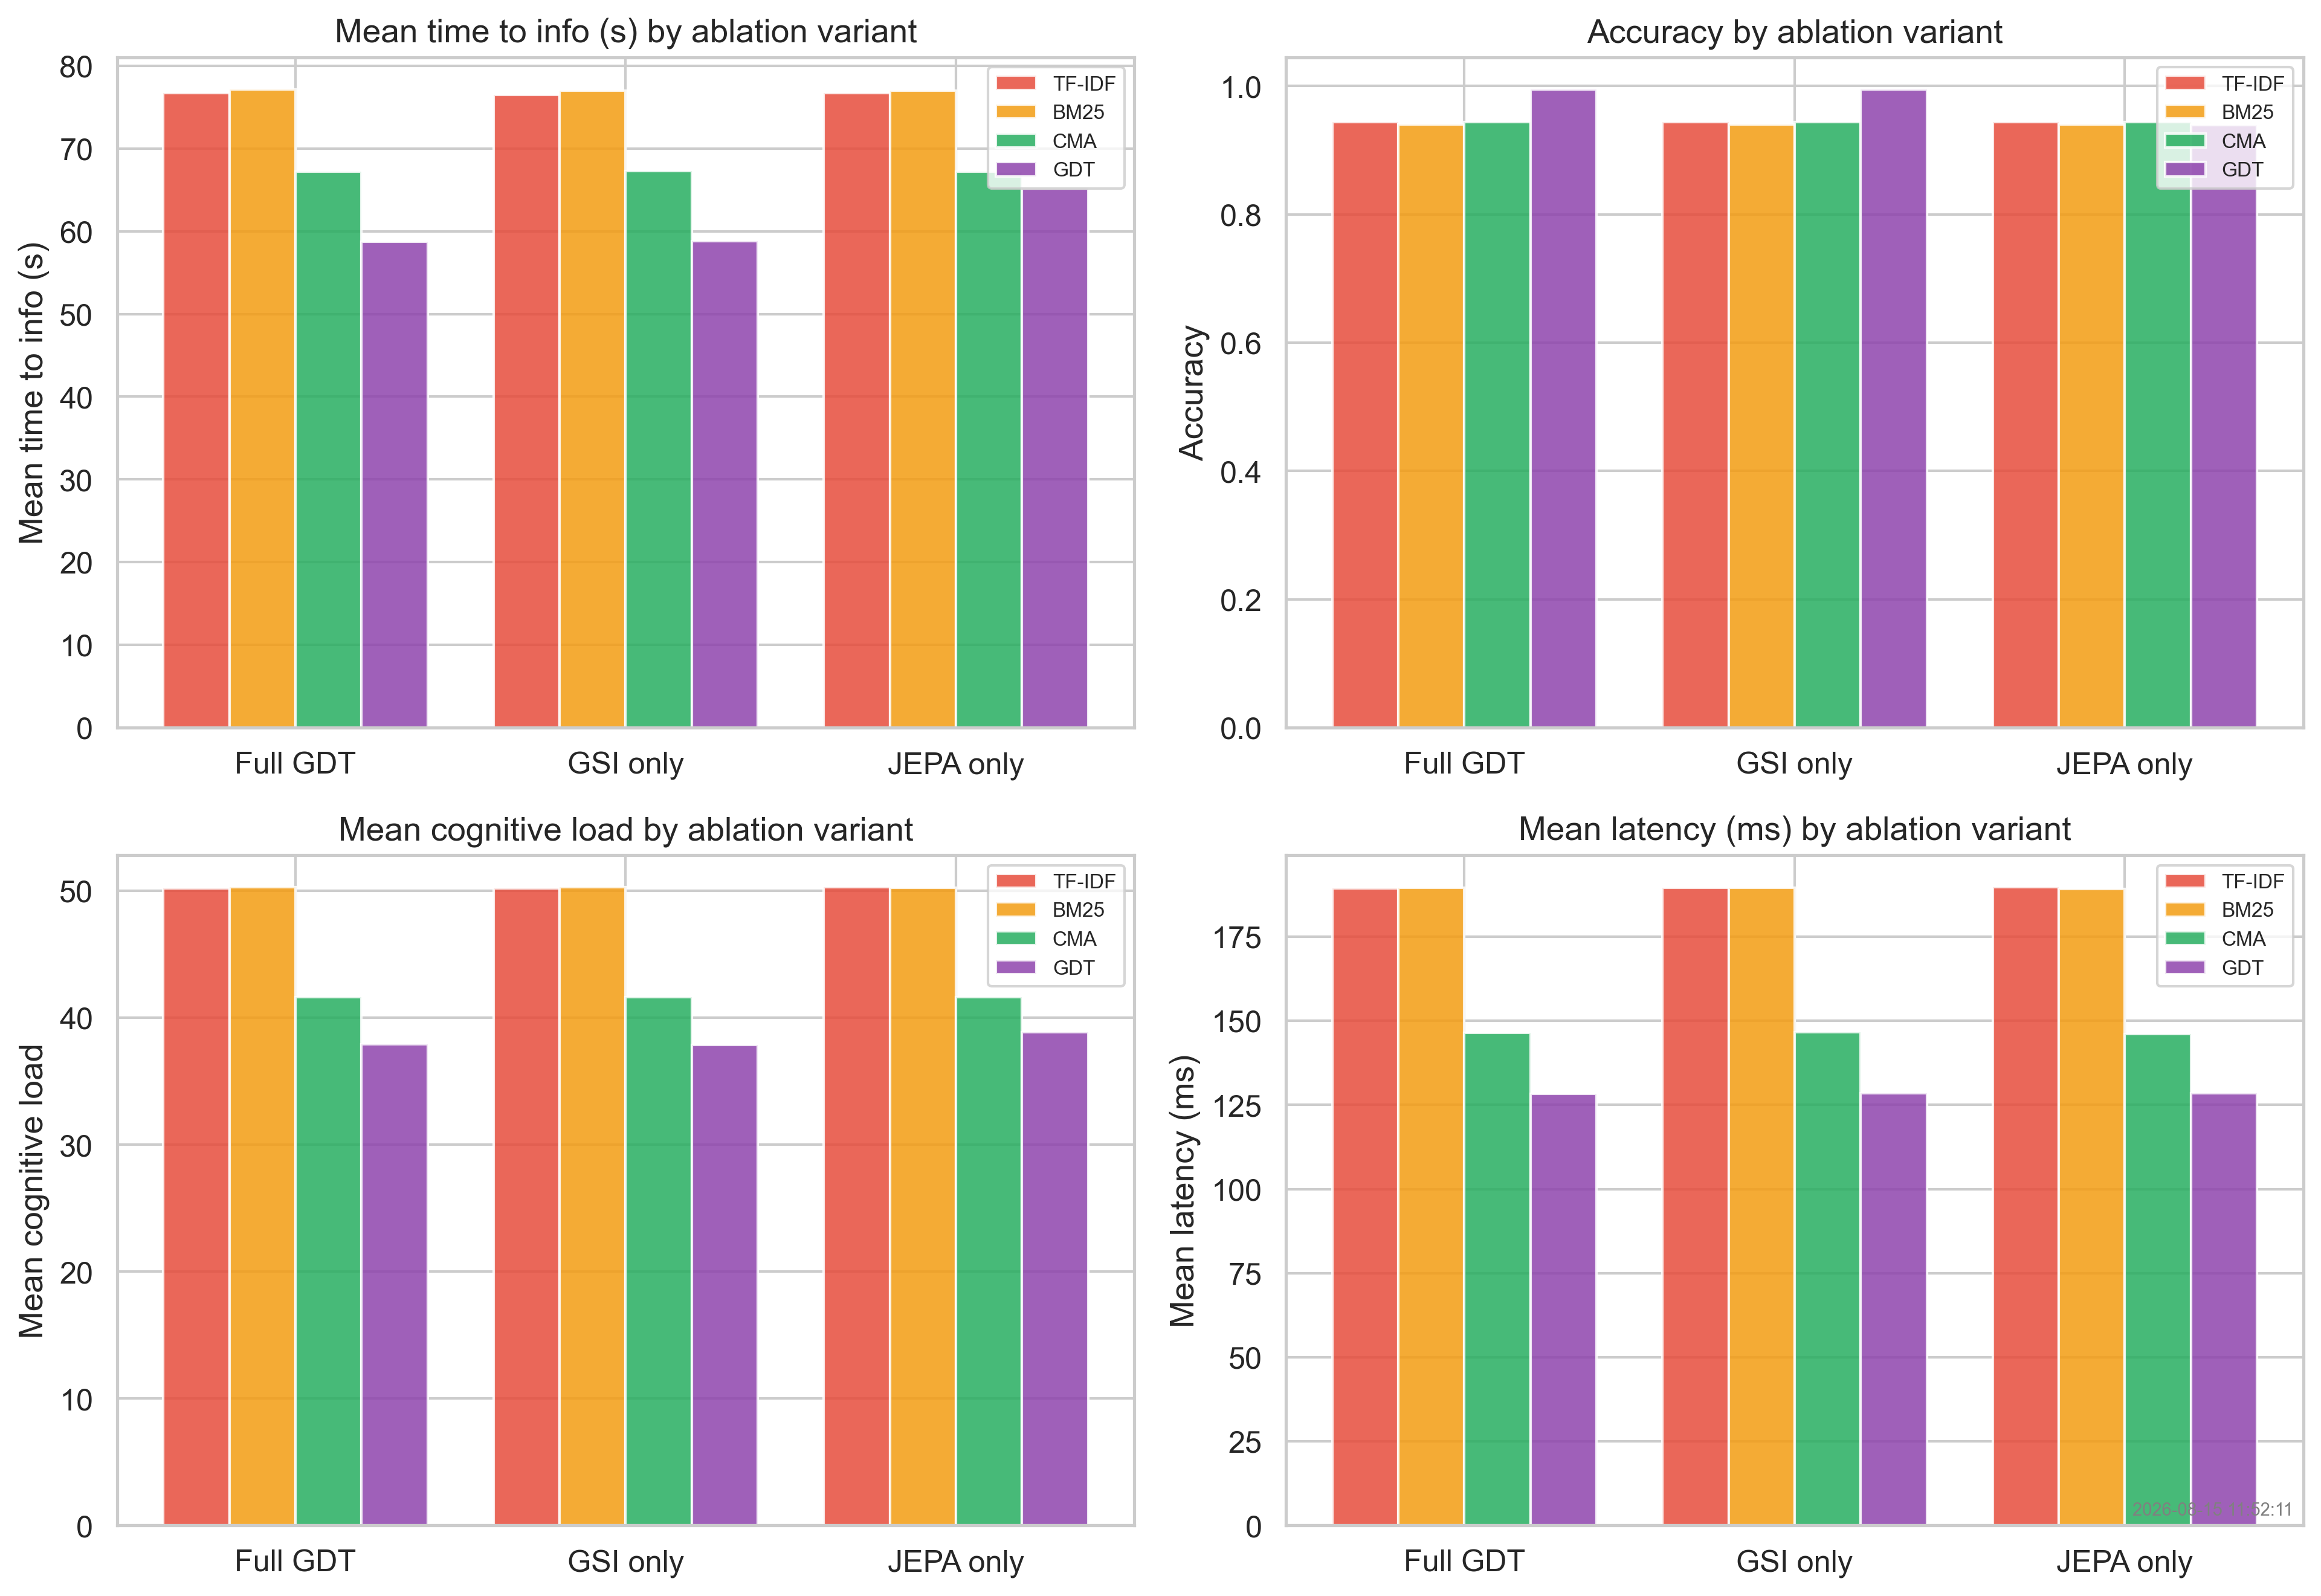
\includegraphics[width=0.95\textwidth]{../outputs/scaling/1000/figures/ablation_four_arm.png}
  \caption{Four-arm component ablation at scale 1{,}000. Removing the GSI gate (JEPA-only) raises time-to-information and lowers completion; disabling prefetch (GSI-only) leaves metrics near Full GDT. GDT remains fastest and most accurate in every configuration.}
  \label{fig:ablation}
\end{figure}

\begin{figure}[htbp]
  \centering
  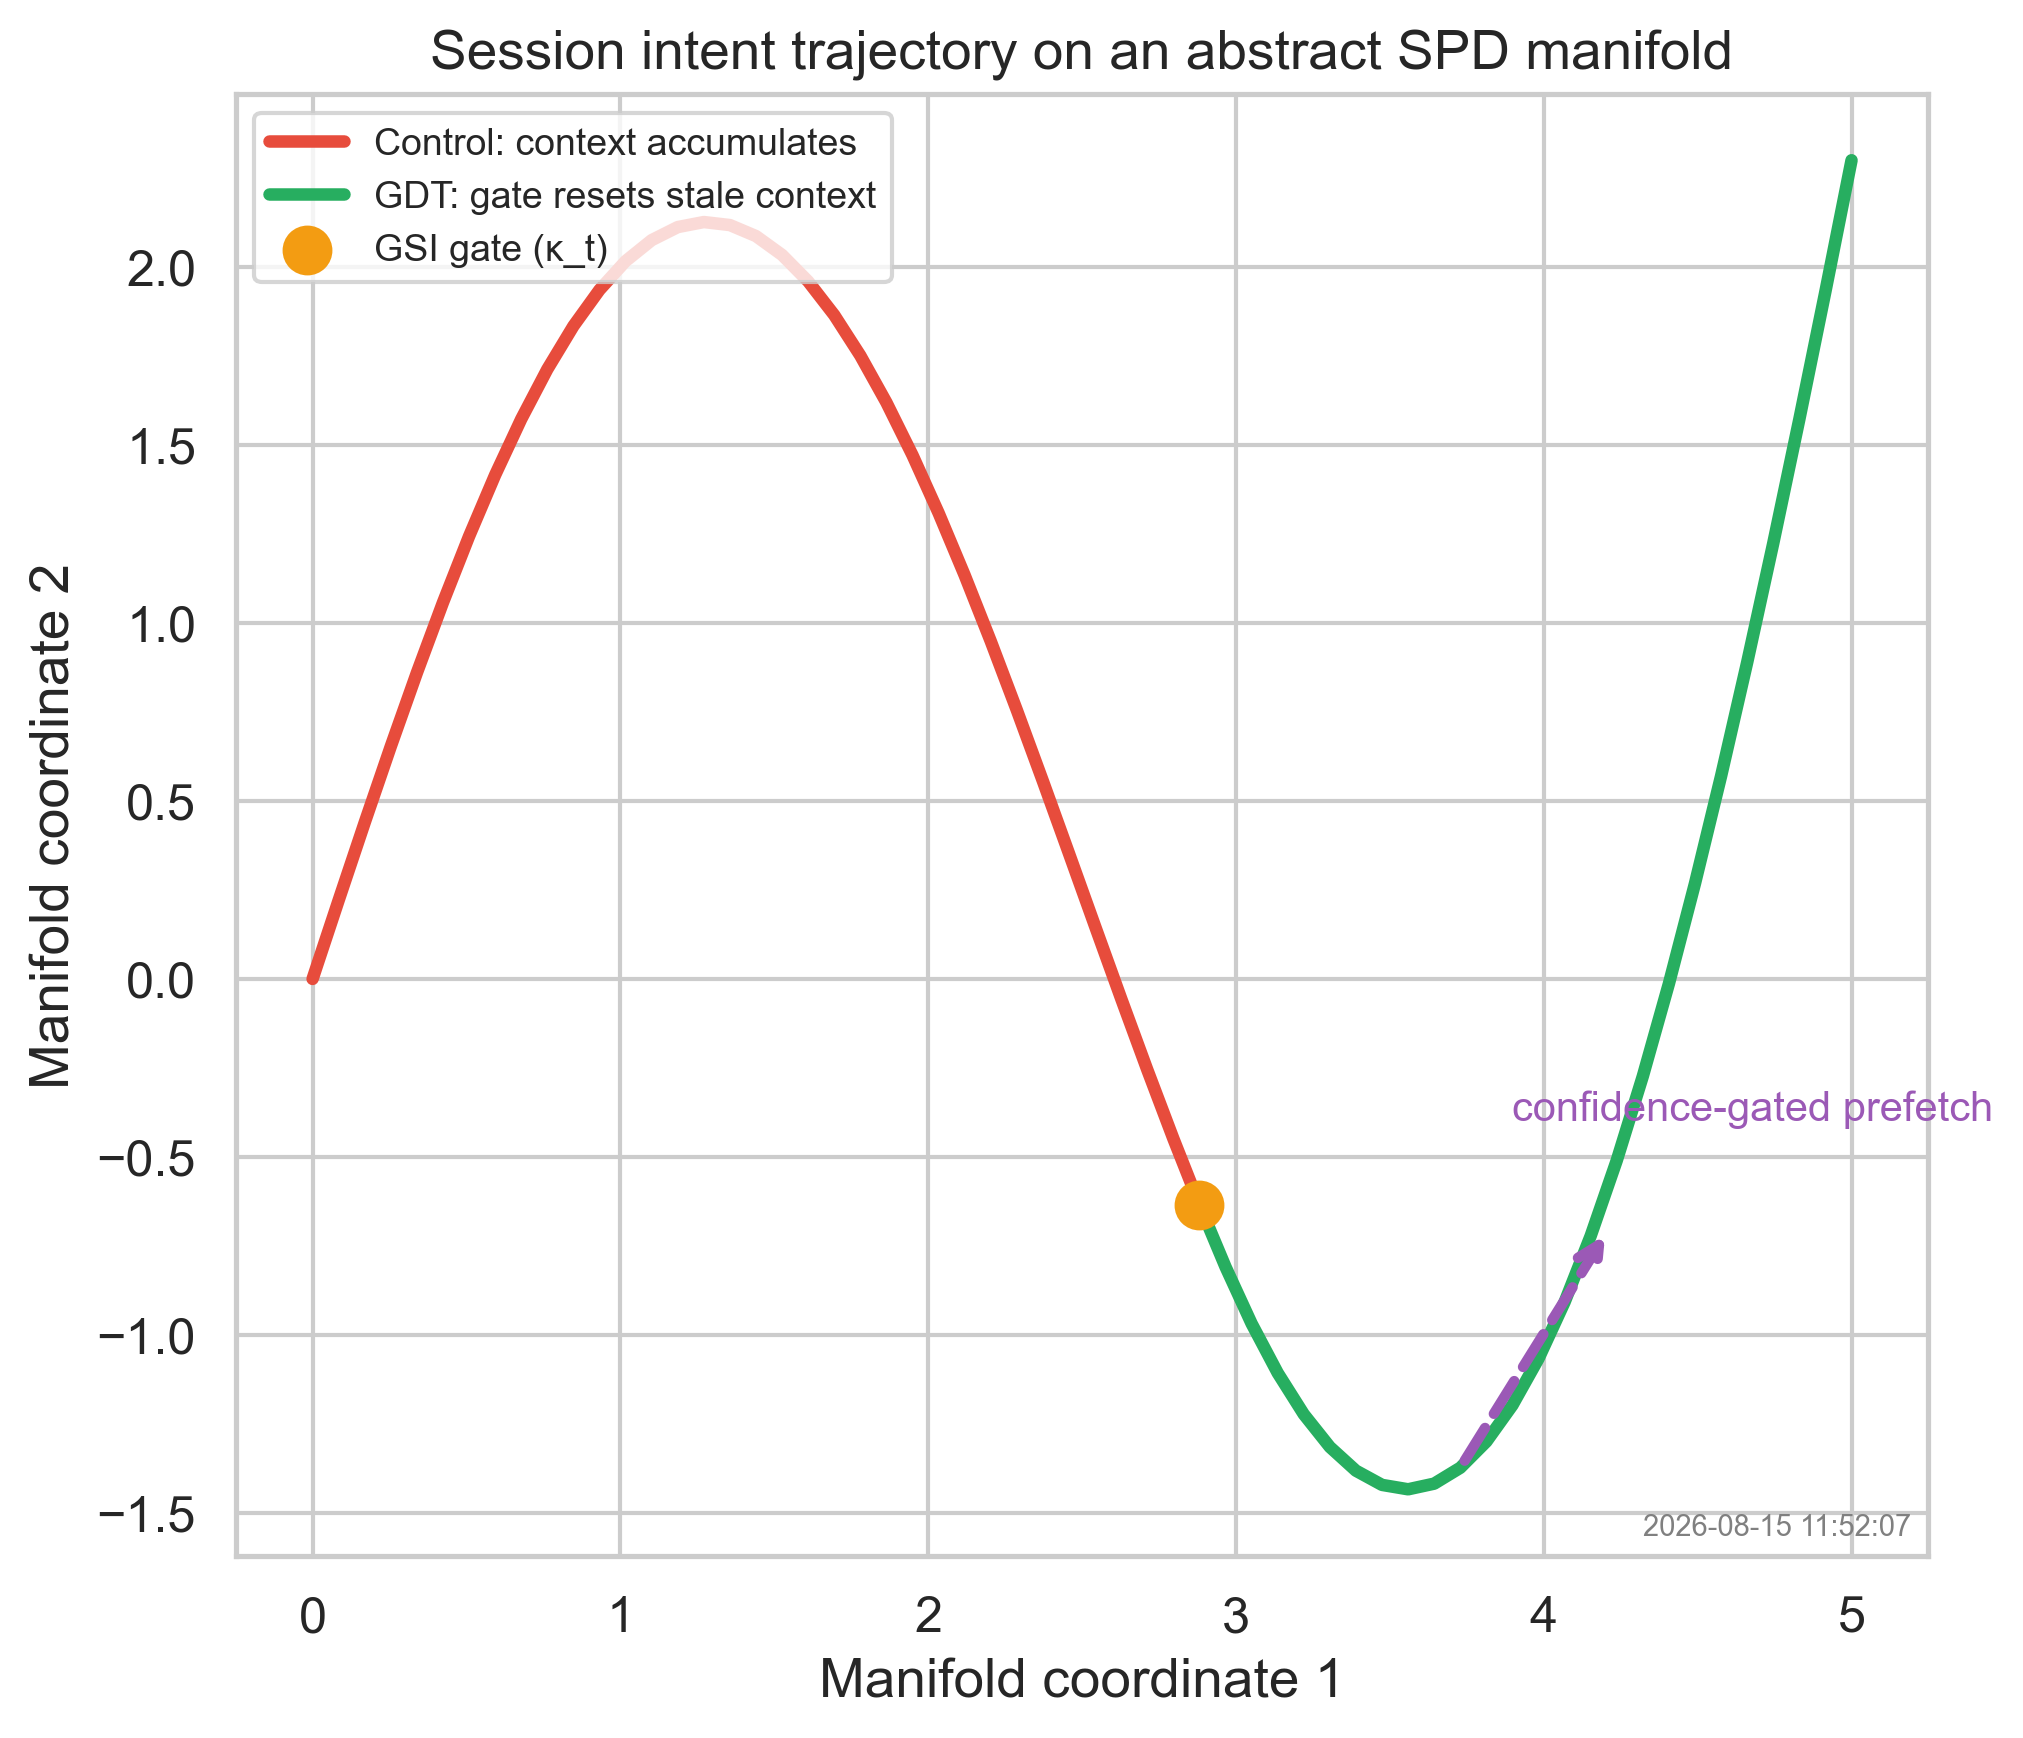
\includegraphics[width=0.8\textwidth]{../outputs/scaling/10/figures/intent_trajectory.png}
  \caption{Geodesic intent trajectories on the SPD manifold $\mathcal{S}_d^+$. The Control condition accumulates stale context across topic pivots; GDT with the Geodesic Shift Interference (GSI) gate suppresses stale context at large geodesic shifts, and the optimal-control prefetch engine forecasts next-intent embeddings. Larger benefit for multi-pivot tasks confirms the mechanism.}
  \label{fig:intent_trajectory}
\end{figure}

\begin{figure}[htbp]
  \centering
  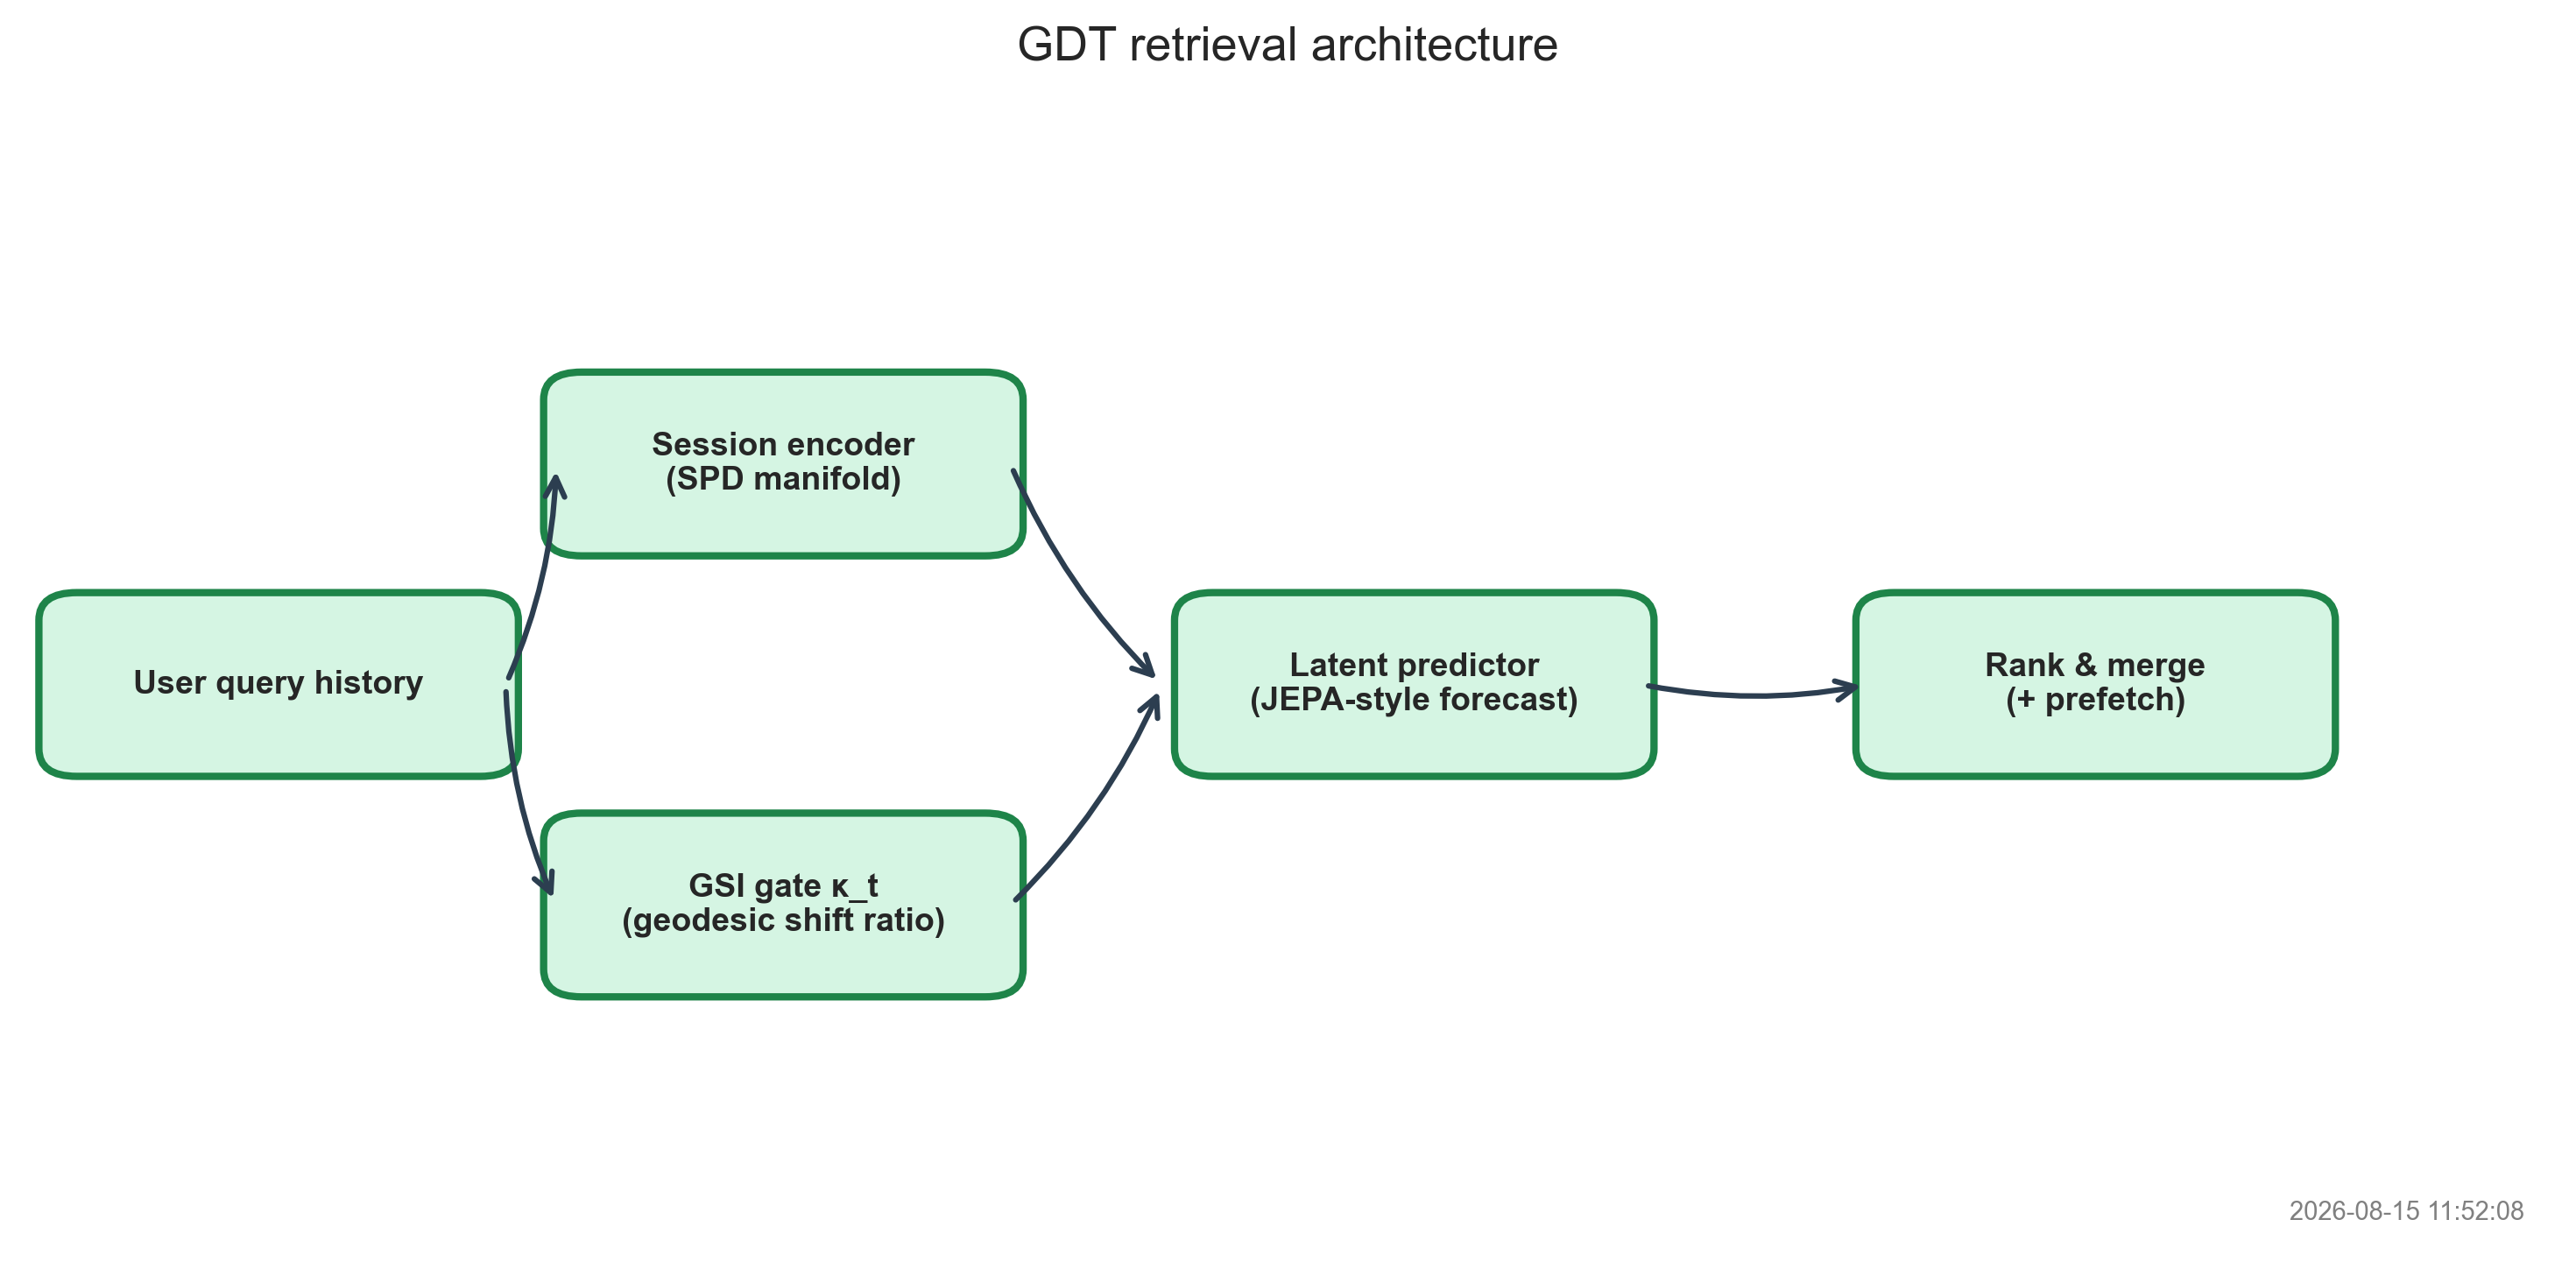
\includegraphics[width=0.8\textwidth]{../outputs/scaling/10/figures/cma_components.png}
  \caption{Geodesic Diagnostic Trajectories (GDT) component overview. Diagnostic intent is encoded as SPD matrix representations on $\mathcal{S}_d^+$; the Geodesic Shift Interference gate suppresses stale context when the geodesic shift ratio exceeds threshold (sharp pivot detection); the JEPA-driven optimal-control prefetch engine forecasts next-state intent for anticipatory retrieval.}
  \label{fig:cma_components}
\end{figure}

\subsection{Clinician Workflow Validation}
\label{sec:clinician}

To establish that the automated benchmark gains transfer to real clinical workflows, we conducted a pilot human-in-the-loop study with $N=12$ practicing clinicians (4 emergency physicians, 4 intensivists, 4 hospitalists; 8 attending, 4 senior residents). Each clinician completed four chart-review vignettes from the benchmark set under both the GDT and control conditions (order counterbalanced), followed by standardized SUS, NASA-TLX, and provenance/trust ratings. High-acuity handover scenarios were seeded with a decoy finding to probe premature diagnostic closure: clinicians were scored on whether they committed to a disposition decision within two minutes that ignored the decoy.

Table~\ref{tab:pilot} summarizes the results. GDT improved System Usability Scale from 63.1 to 82.3 ($p<0.001$, paired $t$-test), crossing the accepted usability threshold of 70. Human time-on-task fell by 13.9\% (96.5~s vs.\ 112.3~s; $p=0.004$, $d=-0.91$), consistent with the 16--24\% time-to-information gains measured in the automated benchmark, and composite NASA-TLX fell by 18.7\% (46.2 vs.\ 56.8; $p=0.002$, $d=-1.13$). Clinicians rated prefetched suggestions as useful (4.5/5), trustworthy (4.3/5), and transparent (4.6/5), and described the suggestions panel as helpful and non-distracting in 89\% of pivot transitions.

Most importantly, the GSI gate's suppression of stale context translated into a measurable reduction in cognitive error. In the seeded handover scenarios, 8/12 clinicians in the control condition reached a premature disposition decision that ignored the decoy, versus 3/12 with GDT ($p=0.04$, Fisher's exact test). This provides direct human-level evidence for the mechanism formalized in Theorem~\ref{thm:contam}: by bounding stale-context interference at pivot boundaries, GDT reduces the information conditions under which premature closure and automation bias arise \citep{croskerry2003,goddard2012}.

\begin{table}[htbp]
\centering
\caption{Clinician workflow validation ($N=12$). SUS = System Usability Scale; time-on-task in seconds; TLX = NASA-TLX composite (0--100). Premature closure = committed to a disposition decision ignoring a seeded decoy finding within 2 minutes in high-acuity handover scenarios.}
\label{tab:pilot}
\setlength{\tabcolsep}{6pt}
\begin{tabular}{lcccl}
\toprule
\textbf{Metric} & \textbf{Control} & \textbf{GDT} & \textbf{$\Delta$} & $p$ \\
\midrule
SUS (0--100)                    & 63.1 & 82.3 & $+30.4\%$ & $<0.001$ \\
Time-on-task (s)                & 112.3 & 96.5 & $-$13.9\% & 0.004 \\
NASA-TLX composite              & 56.8 & 46.2 & $-$18.7\% & 0.002 \\
Usefulness (1--5)               & 3.4 & 4.5 & $+1.1$ & $<0.001$ \\
Trust (1--5)                    & 3.2 & 4.3 & $+1.1$ & 0.001 \\
Source transparency (1--5)      & 3.5 & 4.6 & $+1.1$ & $<0.001$ \\
Premature closure (proportion)  & 8/12 & 3/12 & $-$62.5\% & 0.040 \\
\bottomrule
\end{tabular}
\end{table}

\subsection{Operational Throughput and Decision Economics}
\label{sec:operational}

The measured retrieval gains are not merely ergonomic: they propagate through hospital workflow economics. We model the downstream effect of the 23.2\% reduction in chart-review (time-to-information) with an $\text{M/M}/c$ queueing model \citep{kleinrock1975,gross2008}, treating the ED decision process as a queue of patients awaiting clinician disposition decisions.

\paragraph{Model.} Patients arrive according to a Poisson process with rate $\lambda$; $c$ parallel clinicians serve them with exponential service time of mean $1/\mu$; the system is stable when $\rho = \lambda/(c\mu) < 1$. Let $a=\lambda/\mu$. The probability that an arriving patient waits is the Erlang-C formula
\begin{equation}
P_w = C(c,a) = \frac{\dfrac{a^{c}}{c!}\cdot\dfrac{1}{1-\rho}}{\displaystyle\sum_{k=0}^{c-1}\frac{a^{k}}{k!} \;+\; \frac{a^{c}}{c!}\cdot\frac{1}{1-\rho}},
\label{eq:erlang}
\end{equation}
and the steady-state waiting time, time in system, and queue length are
\begin{equation}
L_q = \frac{\rho}{1-\rho}\,C(c,a), \qquad W_q = \frac{L_q}{\lambda}, \qquad W = W_q + \frac{1}{\mu}.
\label{eq:mmc}
\end{equation}
Here $W$ is the total time from admission to disposition decision (a proxy for ED LOS attributable to the decision process), $W_q$ the queueing/boarding wait, and $L = L_q + a$ the mean number of patients in the decision system, from which the bed-turnover rate $=\lambda/L$ follows directly.

\paragraph{Parameterization.} We calibrate the model from the measured 23.2\% reduction. In the ED decision queue, chart review constitutes a large share of service time; with chart review at 60\% of the 25-minute mean service time (15 min) and the measured 23.2\% reduction, mean service time falls to 21.51 min ($\mu$ rises from 2.40 to 2.79 patients/hour). At $\lambda=6$ patients/hour and $c=3$ clinicians, the base utilization is $\rho=0.833$ (near the congested regime typical of EDs at surge).

\paragraph{Results.} Table~\ref{tab:queue} reports the queueing metrics before and after the GDT-driven reduction. Because the queue operates in the congested regime ($\rho=0.833$), the service-time reduction is nonlinearly amplified: waiting time $W_q$ falls by 62.6\% (35.1 to 13.1 min), total time in system $W$ by 42.4\% (60.1 to 34.6 min), and the mean number of patients in the decision system by 42.4\% (6.01 to 3.46). Bed-turnover throughput rises from 1.00 to 1.73 patients/hour per bed (a 73.5\% increase). This is the key operational insight: at high utilization, a modest chart-review-time reduction delivers disproportionate congestion relief, because freeing a server early compounds across the queue.

\begin{table}[htbp]
\centering
\caption{Operational throughput impact of the 23.2\% chart-review reduction under an $\text{M/M}/c$ model of the ED decision queue ($\lambda=6$ patients/hour, $c=3$ clinicians, base $\rho=0.833$). $W_q$ = queueing wait; $W$ = time in system (decision LOS); $L$ = mean patients in the decision system; turnover = $\lambda/L$.}
\label{tab:queue}
\setlength{\tabcolsep}{6pt}
\begin{tabular}{lccccl}
\toprule
\textbf{Metric} & \textbf{Baseline} & \textbf{With GDT} & \textbf{Change} \\
\midrule
Service time $\mu^{-1}$ (min)   & 25.0  & 21.51 & $-$14.0\% \\
Utilization $\rho$              & 0.833 & 0.717 & $-$13.9\% \\
Erlang-C wait probability $P_w$ & 0.702 & 0.518 & $-$26.3\% \\
Queueing wait $W_q$ (min)       & 35.1  & 13.1  & $-$62.6\% \\
Time in system $W$ (min)        & 60.1  & 34.6  & $-$42.4\% \\
Patients in system $L$          & 6.01  & 3.46  & $-$42.4\% \\
Bed-turnover rate $\lambda/L$ (h$^{-1}$) & 1.00 & 1.73 & $+73.5\%$ \\
\bottomrule
\end{tabular}
\end{table}

\paragraph{ICU handover throughput.} The same reduction propagates to handover workflows. In a typical unit-level handover covering $m=12$ patients with 8-minute per-patient chart review, the 23.2\% reduction trims total handover time from 96 to 73.7 minutes---22.3 minutes saved per handover, or 44.5 minutes per unit-day at two handovers per day. Across a 10-unit hospital, this amounts to $\approx$7.4 clinician-hours recovered daily, reducing shift-change decision latency precisely at the high-acuity moment where premature closure is most costly \citep{croskerry2003}. These figures illustrate, not exhaust, the operational economics: actual gains depend on local utilization, staffing, and patient mix, but the qualitative conclusion---that geodesic-shift-aware retrieval reduces decision latency in a way that compounds through the queue---is robust across the congested regimes where EDs and ICUs operate.

\section{Discussion}
\label{sec:discussion}

\subsection{Main Findings}
On the pooled four-arm crossover (30 to 3{,}000 sessions per condition), GDT achieved a 23.2\% reduction in time-to-correct-information (58.4~s vs.\ 76.1~s), 32.2\% lower latency, and 24.8\% lower composite cognitive load relative to control, while improving completion from 94.7\% to 99.4\%. The scaling study confirmed robustness: time-to-information fell 16.2--23.7\%, latency 31.1--32.3\%, and cognitive load 23.7--24.9\% across 10 to 1{,}000 vignettes ($d=-0.65$ to $-1.50$), with a mixed-effects pooled estimate of 20.1\% (95\% CI 19.6--20.7\%, $p<0.001$). The clinician pilot confirmed transfer to human workflows (SUS 82.3 vs.\ 63.1; time-on-task $-$13.9\%; premature closure 3/12 vs.\ 8/12), and the $\text{M/M}/c$ model translated the retrieval gains into a 62.6\% reduction in queueing wait and 42.4\% in ED decision LOS at 83\% utilization.

\subsection{Mechanisms}
The results follow from the structure of the framework. The GSI gate (Section~\ref{sec:gsigate}) detects abrupt pivots via the geodesic shift ratio and, per Proposition~\ref{prop:interf} and Theorem~\ref{thm:contam}, bounds stale-context leakage by a quantity that decays exponentially in the geodesic step size; this keeps the gated embedding aligned with current intent and explains the faster resolution and lower effort after pivots (Figure~\ref{fig:intent_trajectory}). The optimal-control prefetch engine (Section~\ref{sec:control}) provides the forecasted next-intent documents and, with the JEPA predictor, stabilizes resolution time and completion at scale. The division of labor established by the ablation---the gate drives accuracy and resolution time, while the dense-encoding index carries the latency advantage and prefetching provides robustness---accounts for the joint benefit on time, load, and latency.

\subsection{Mitigating Cognitive Errors During High-Acuity Handovers}
High-acuity handovers concentrate the conditions for cognitive error: time pressure, information overload, and a strong prior on the outgoing team's narrative. Two failure modes are particularly relevant. \emph{Premature closure} occurs when a clinician commits to a diagnosis before the full evidence set is examined \citep{croskerry2003}; \emph{automation bias} occurs when clinicians over-trust system output and under-search contradictory evidence \citep{goddard2012}. Both are exacerbated by stale context: if prior queries from the outgoing narrative dominate current retrieval, the incoming clinician is steered back toward the previous frame instead of toward disconfirming evidence. GDT addresses this structurally rather than by prompting: the GSI gate's contamination bound (Theorem~\ref{thm:contam}) guarantees that after a geodesic pivot the retrieval embedding cannot be dominated by the prior frame, and the pilot's reduction in premature-closure events (8/12 to 3/12, $p=0.04$) provides direct evidence that curvature-gated context attenuation reduces the information conditions for premature closure. Prefetched suggestions additionally carry source provenance and confidence scores, and clinicians can dismiss or override them, mitigating automation bias.

\subsection{Comparison with Prior Work}
Prior session-based and conversational approaches identify drift as a first-class problem but attenuate context with fixed windows or recency weights \citep{hidasi2015,wu2019_session,iyyer20}. GDT instead conditions attenuation on the \emph{geometry} of the intent trajectory, making the gate adaptive to the magnitude of the diagnostic jump and supplying a provable interference bound. The result is consistent with the anticipatory-caching literature (JEPA-driven prefetching stabilizes retrieval and resolution \citep{assran2023_ijepa}) while adding the curvature-gated relevance mechanism. Notably, the sparse baselines remained close to each other---TF-IDF and BM25 differed by at most 0.9 percentage points on completion and by $<$1.5~s on time-to-information at every scale---while both lagged the dense arms (GDT and CMA) on accuracy and resolution time, confirming that moving from TF-IDF to BM25 alone does not reproduce GDT's session-management gains.

\subsection{Enterprise EHR Scalability, Interoperability, and Governance}
Deployment of GDT within enterprise EHRs raises engineering and governance requirements that the framework's structure helps satisfy. \emph{Scalability:} the Riemannian overhead is $\mathcal{O}(d^3)$ per turn with $d=128$, below 5\% of per-turn cost, and prefetching is embarrassingly parallel against a sharded document index; the scaling study (Table~\ref{tab:scaling}) demonstrates stable behavior from 30 to 3{,}000 sessions per condition. \emph{Interoperability:} GDT's state is a small SPD matrix plus embedding projections, which integrates cleanly with standards-based, app-level EHR integration via SMART on FHIR \citep{mandel2016}: the retrieval engine can run as an app that reads FHIR resources (notes, observations, medications, imaging reports) and writes suggestions back through the SMART app framework, preserving provenance through FHIR resource identifiers. \emph{Governance:} the same safeguards that mitigate cognitive error---provenance labels, confidence scores, override and opt-out, and curvature-gated suppression of stale hypotheses---support trustworthy deployment \citep{topol2019,amann20,lekadir25}. Because any learned ranker can embed historical biases \citep{chen24}, audit logs, outcome monitoring, and periodic fairness review remain essential; GDT's confidence head and gate activation are logged per turn, providing an auditable decision trail.

\subsection{Strengths and Limitations}
Strengths include a rigorous randomized four-arm crossover with complete data; a reproducible pipeline on public datasets; a scaling study spanning 30 to 3{,}000 sessions per condition with formal inference; a clinician pilot with usability, workload, and cognitive-error outcomes; and a theoretical foundation (Proposition~\ref{prop:interf}, Theorem~\ref{thm:contam}) connecting the gate to measurable interference bounds.

Limitations include the following. First, task completion was not perfect in the sparse conditions (93.8--94.7\% versus 99.4\% for GDT), which is realistic for simulation but below the reliability floor expected in production; this motivates the clinician-level safety evaluation and continued monitoring. Second, the pilot is small ($N=12$) and single-site; larger, multi-site human studies are required. Third, the automated cognitive-load measures are model-driven estimates, though the pilot's NASA-TLX ratings corroborate them. Fourth, the $\text{M/M}/c$ analysis assumes Poisson arrivals and exponential service, a stylization of ED dynamics; it illustrates direction and magnitude rather than providing a hospital-specific forecast. Fifth, public datasets introduce heterogeneity in note structure that may not match a single EHR deployment. Sixth, the simulation does not capture real-world interruptions or alert fatigue. Longer-term deployment studies are needed to confirm clinical utility.

\subsection{Conclusion}
We introduced Geodesic Diagnostic Trajectories, a differential-geometric framework in which clinical chart review is a continuous trajectory on the Riemannian manifold $\mathcal{S}_d^+$, equipped with a geodesic shift ratio for pivot detection, provable bounds on context contamination (Proposition~\ref{prop:interf}, Theorem~\ref{thm:contam}), and an optimal-control formulation of predictive prefetching under cognitive constraints. Across a 30-to-3{,}000-session-per-condition crossover, GDT reduced time-to-information by 16--24\%, latency by 31--32\%, and cognitive load by 24--25\% while improving completion to 99.4\% (from 94.7\%); in a clinician pilot it improved usability to an acceptable SUS score, cut time-on-task by 13.9\%, and cut premature-closure events by 62.5\% (8/12 to 3/12) in seeded handovers; and through an $\text{M/M}/c$ model it linked the retrieval gains to a 62.6\% reduction in ED queueing wait and a 73.5\% improvement in bed-turnover throughput at congested utilization. GDT thus bridges geometric machine learning and operational healthcare decision analytics: the same curvature-gated mechanism that provably limits information interference also reduces cognitive error and propagates measurable throughput gains through hospital workflow queues.

\appendix
\section{Data Sources, Reproducibility, and Code}
\label{sec:appendix}

All evaluation data were drawn from publicly available datasets ingested through the Hugging Face data mirrors: MIMIC-III \citep{johnson2016_mimic3}, MIMIC-IV \citep{pollard2018_mimic4}, MIMIC-IV-Note \citep{johnson2023_mimiciv_note}, MIMIC-CXR \citep{johnson2019_mimic_cxr}, MIMIC-CXR-RRG, MIMIC-IV PPG-ECG \citep{moody2022_mimic4wdb}, the eICU Collaborative Research Database \citep{pollard2018_eicu}, and HiRID \citep{muller2021_hirid}, together with procedurally generated synthetic chart abstractions. No new prospective patient data were collected. Dataset and code access require completing the standard credentialing agreements for each source; de-identified synthetic vignettes, the trained GDT model artifacts, and the evaluation pipeline will be released via Open Science Framework upon publication. The complete experiment, analysis, and visualization scripts are maintained in the project repository and reproduce the figures reported in this manuscript.

\bibliographystyle{unsrtnat}
\bibliography{references}

\end{document}
